%# -*- coding:utf-8 -*-
%!TEX root = ../thesis.tex

\chapter{水下机器人的驱动补偿控制 }

\label{chap:actuator_nonlinearities}
% 6.1 引言
% 6.2 现代补偿器描述
% 6.3 带有补偿器的模型参考自适应控制
% 6.4 带有补偿器的L1AC 自适应控制
% 6.5 仿真结果与分析
% 6.6 本章小结
\section{引言 }

随着技术的发展水下航行器已经被广泛用于水下油气管道勘测以及海洋探测活动中,这为实际的水下航行器的系统开发带来了很大的挑战。水下机器人的开发受到的影响因素主要包括系统动力学、导航性能、运动控制及路径规划的能力。其中对于导航和路径规划功能的实现,都是要依靠航行器的控制器的来实现\cite{richter2016polynomial}。水下机器人工作的环境使得水下机器人的系统动力学具有很强的非线性与多自由度耦合性。上一章研究的鲁棒自适应控制不仅可以处理模型的不确定性问题,也可以保证控制系统的稳定性。然而,鲁棒自适应控制器根本上还是一种状态反馈控制,在适应模型的不确定时,主要是通过改变控制器的增益来实现,这样的控制器不仅耗费较多的能量,而且忽视了水下机器人系统中动态特性。

水下机器人可以自行适应干扰,但是水下机器人的系统并不善于利用系统本身的动态特点来辅助水下机器人进行运动。对于静不平衡鱼雷型水下机器人,控制面舵的工作物理空间是受到限制的,而状态控制器给出的控制指令是在受限制的空间内进行选取驱动输入的。控制面舵的物理工作空间对于水下机器人是否都高效率呢?类似于人类行走或者鱼类尾部摆动,日常的活动所需要的步幅和尾部摆动幅度并不是全空间内进行改变的,而是有个主要的工作范围。对于水下机器人而言,控制面舵的主要工作空间是否可以主要利用部分区域就可以实现控制目标?

水下机器人的控制较为复杂,其自身特点也兼有非线性、耦合性。自适应控制要解决的主要问题就是模型的不确定性和系统中的未建模的非线性部分。鲁棒自适应控制可以让控制器追求鲁棒性、稳定性和响应的速度,但是鲁棒自适应控制并不能利用蕴含在水下机器人系统中的动态特性来改善控制器的性能。控制面舵的阈值特性是本章要解决主要的问题之一,不过驱动器的死区、时间延迟等问题也需要重视。本章将对驱动器的非线性动态特性进行系统说明,并给出数学模型描述。要应对系统动态特性带来的控制挑战,需要重新评价并改善鲁棒自适应控制框架尤其是模型参考自适应控制与$L_1$自适应控制的性能。鲁棒自适应控制不仅要应对模型参数不确定性,还应考虑驱动器带来的输入饱和以及高效动态空间的特点。抗饱和补偿器被设计出来用于解决输入非线性的问题。补偿器是一种辅助设计控制器,可与别的控制方法进行组合。文中主要选择使用Riccati抗饱和补偿器,并将其分别与投影模型参考自适应控制和$L_1$自适应控制器进行融合。根据上一章的研究,$L_1$自适应控制方法与MRAC控制相比,具有很大的优势,因为其自适应的功能实现不需要牺牲控制器的响应速度。$L_1$自适应控制在控制性能与参数更新方面优于模型参考自适应控制。本章将从利用系统动态的角度继续对比两种自适应控制方法,从而更好地发掘控制器的潜力。

本章研究的对象是REMUS AUV,该型水下机器人的模型具有非线性、耦合性、静不稳定性。REMUS的水中浮力大于重力,导致系统在水中不能处于静止悬浮状态,系统的不稳定会给别的自由度如俯仰、偏航姿态控制带来影响。将带有驱动补偿的鲁棒自适应控制方法分别应用于水下机器人的姿态控制与深度控制问题中,分别使用线性系统、6自由度耦合模型验证方法的有效性。从利用控制面舵的有效工作空间的角度,给出带有驱动补偿器的鲁棒自适应控制方法对于系统耦合问题的使用前后的性能对比。

% 最后,给出水下机器人的LOS轨迹引导律,并对比期望轨迹与实际运行轨迹,以充分验证所提出方法的可行性。



\section{水下机器人的驱动器非线性 }

实际水下机器人的驱动器是具有自身的特性,但是在很多控制中会将驱动的动态特性忽视。本节主要研究水下机器人的驱动器的系统特性,并给出各个动态特性的数学模型。首先从水下机器人中常用的驱动器类型确定控制面舵、无刷电动直流电机为主要研究的对象。无刷直流电机的驱动器是使用电调驱动的,通常使用PWM脉冲信号来控制。对于正反电调驱动无刷电机类型的推进器,输入信号是有最大值和最小值要求的,即阈值;此外,信号正反转启动信号之间有一段驱动是无效的,即为死区。对于控制面舵(水面舵和垂直舵),舵片的舵角是在物理空间内受到限制的,因此舵片的系统动态输入具有阈值特性。水下机器人的驱动器收到的控制指令有时并不是实时的,可能由于水面控制信号传输或者系统本身使得驱动器接收的命令具有延迟特性。

\subsection{输入阈值 }

水下机器人的驱动器有控制面舵和推进器。控制面舵的物理控制空间是受到限制的,因此当计算的控制输入达到阈值边界,就会影响整体的控制性能。推进器的推力也是有最大最小值的,推进器的推力非线性会导致系统控制器变得不稳定,使得系统耗散太多的能量来跟踪控制指令。

控制输入的阈值如图所示,可以将阈值描述成如下形式:
\begin{equation}
\label{eq:chap6:sat}
\delta_r=sat(u)
\end{equation}
式中,$u$ 是控制器计算的值,$\delta_r$ 是驱动器实际接收到值,$sat()$ 表示非线性的阈值特征。

可以进一步写成如下形式:

\begin{equation}
\label{eq:chap6:sat}
\delta_r=sat(u)=
\left\{
\begin{matrix}
  \delta_{rm} & u > \delta_{rm}\\
   u & -\delta_{rm} \leq u \leq \delta_{rm}\\
   -\delta_{rm} & u < -\delta_{rm} \\
\end{matrix}\right.
\end{equation}
式中,$\delta_{rm}$ 是驱动器的阈值上边界。

\begin{figure}[!htp]
\centering
 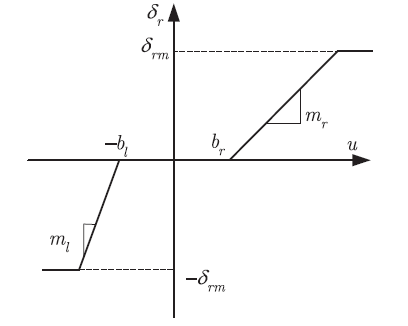
\includegraphics[width=8cm]{figure/chap6/sat.png}
 \label{fig:chap6:F1}
 \bicaption[fig:chap6:F1]{驱动器阈值}{驱动器阈值} {Fig.}{Actuator saturation}
\end{figure}

\subsection{死区 }

推进器和控制面舵的控制信号并不是连续有效的。在某一个区间内,控制信号的输入是不能驱动电机的,因为无刷直流电机的驱动电调是有截止范围,具体可以见图\ref{fig:chap6:F1}。在不考虑阈值时,驱动器的信号死区的数学表达式如下:

\begin{equation}
\label{eq:chap6:sat}
\delta_{r} = \left\{
\begin{matrix}
0  ,&  u_{bl} \leq u \leq u_{br}  \\
k_{bl}u + \delta_{bl} ,&   u \leq u_{bl} \\
k_{br}u + \delta_{br} ,&   u \geq u_{br} \\
\end{matrix}\right.
\end{equation}
式中,$u_{br}$ 和 $u_{bl}$ 分别为驱动器的死区的上下界。$k_{br}$ 和 $k_{bl}$ 分别为驱动器输入信号的斜率。

对于无刷电机推进器,其系统兼有死区与阈值特性,而对于控制面舵,主要的系统特性是阈值。本章研究的鱼雷型水下机器人的姿态控制是依靠控制面舵片实现的,因此本章将主要研究控制面舵的阈值特性的动态补偿问题。

\subsection{时间延迟 }

不同的水下机器人的通信方式以及驱动器类型是不同的,对于遥控式深海水下机器人,有时因为上下位机的信号传输会给驱动器执行带来时间上滞后,另外有些驱动器的本身也具有时间延迟特点,从控制信号输入到驱动器产生驱动力的过程并不是瞬时的,有一个 $\Delta t$的时间滞后。带有时间延迟的水下机器人的状态方程形式的系统模型表示如下:
\begin{equation}
\label{eq:chap6:sat}
\begin{aligned}
 \dot x(t) &= A x(t) +  B \Lambda u(t - \Delta t) \\
 \dot y(t) &= C^T x(t)\\
\end{aligned}
\end{equation}
式中,$x$ 是系统的状态量, $A$ 是系统的状态传递矩阵, $B$ 是控制常数矩阵, $\Lambda$ 是正定义矩阵,$y(t)$ 是系统的测量输出, $C$ 是测量的传递矩阵。

时间延迟在许多系统中都会出现,会导致控制系统不稳定或者降低系统的工作性能。水下机器人中的驱动器的执行也可能会出现时间延迟问题,这对于工作于未知水下环境中的航行器的稳定带来诸多挑战,因此在进行控制系统设计时也要对带有延迟的水下机器人系统工作稳定情况进行分析并测试控制器的工作性能。常用的时间延迟系统的系统分析方法有Lyapunov法、耗散分析法、线性矩阵不等式分析法\cite{yuli2002,feng2016dissipativity,feng2015reachable}。

\section{现代补偿器}
当控制器计算的期望输出大于驱动器的本身能力时就会出现驱动阈值问题。大多数的情况下,工业系统的设计是假设驱动器能力是足够的,但是这样的设计会给系统的成本和性能都带来更高的要求。另外,这样的假设也会在系统的利用效率上出现问题。水下机器人这类系统也容易出现阈值问题,如果开发系统的潜力并着重利用现有的驱动器来实现目标,这将是有益的。不仅可以降低成本,也可以节省能量。研究者一直在搜寻解决阈值问题的方法,很多人关注了驱动器达到阈值时的饱和问题,例如性能、系统稳定性。最初的大多数的阈值问题的解决方法缺乏正式的稳定性保证,后来出现现代抗饱和补偿方法实现了这一目标。当阈值情况出现时,从工业的角度来看,饱和是引起系统性能下降的原因。这也传递这样的事实,当阈值情况未出现时,控制器的输出就是“不受限制的响应”,这时理想的输出与控制器的输出是重合的。当阈值情况出现时,抗饱和控制器的响应输出应当尽可能地接近“不受限制的响应”。
\subsection{基本的抗饱和框架 }

水下机器人系统的非受限制控制器是在没有驱动器饱和问题的条件下进行设计,获得的控制器能够保证闭环稳定性。在进行抗饱和控制设计时,也是假设非受限制控制器是闭环稳定的。对于足够小的控制信号,驱动器的阈值的作用就像是个单位矩阵,这样带有阈值特性的闭环系统的近似稳定性是可以得到保证的。如此,可以将阈值的影响以及抗饱和的校正作用视为一种增量行为,而这种行为在非饱和系统中是没有的。基于这个思想可以得到抗饱和的基本框架,如图\ref{fig:chap6:F2}。图中,线性闭环系统被阈值的输入输出信号之间的差值,$d(y_c) = sat(y_c) - y_c$,所干扰和影响,在这个框架中,抗饱和过滤器就是利用这个偏差信号来进行校正。

\begin{figure}[!htp]
\centering
 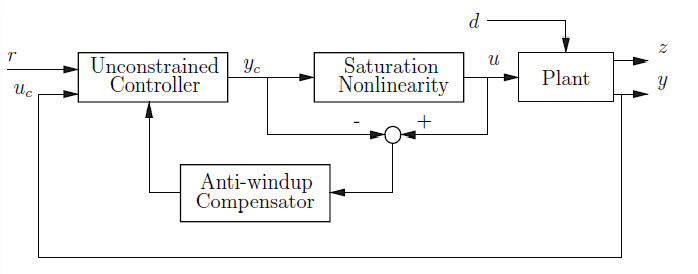
\includegraphics[width=14cm]{figure/chap6/basic_anti-windup.png}
 \label{fig:chap6:F2}
 \bicaption[fig:chap6:F2]{基本的抗饱和控制框架}{基本的抗饱和控制框架} {Fig.}{Basic framework of Anti-windup controller}
\end{figure}

图\ref{fig:chap6:F2}是非常有帮助的,因为图中的补偿器能够自动区分开实际闭环阈值响应与非受限制从闭环响应之间的不一致。当阈值饱和没有被触发时,抗饱和补偿器的输入值为零,这样闭环系统就具有稳定性。因为当非限制控制器的输出为小信号时,补偿器具有自我保持局部近似稳定的能力。此外,图中的模块(plant、controller、anti-windup compensator)可以是线性的或者非线性的,这样就可以对多种不同的系统进行抗抗饱和问题研究。不过在大多数的控制设计中,都是假设系统是线性的。水下机器人尤其是REMUS AUV 这种机器人的系统是具有强非线性的,本章的研究主要是为了解决航行器的非线性系统的饱和问题,下面将给出本文研究的抗饱和补偿器。



\subsection{基于Riccati方程的抗饱和补偿器 }

抗饱和补偿器的主要作用是当阈值饱和条件被达到时,可以快速而平稳的恢复系统。有很多种方法被用来解决这个问题,但是一般、系统且直观有效地成功解决抗饱和问题的并不多。补偿器可以和多种控制结合,而随着结合控制方法的不同,获得的补偿框架也略微不同,下面给出鲁棒控制的补偿器控制结合框图。

\begin{figure}[!htp]
\centering
 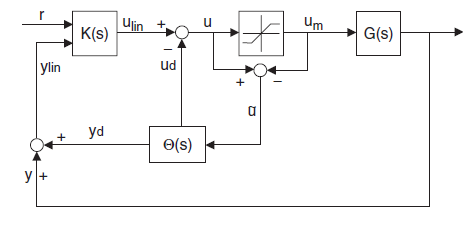
\includegraphics[width=14cm]{figure/chap6/robust_control_AW.png}
 \label{fig:chap6:F3}
 \bicaption[fig:chap6:F3]{鲁棒控制的抗饱和控制框架}{鲁棒控制抗饱和控制框架} {Fig.}{Framework of robust control with anti-windup compensator}
\end{figure}

图\ref{fig:chap6:F3}中,$G(s)$ 是前面框图里提到的系统(plant), $K(s)$ 是用来稳定名义无阈值限制系统并获得理想性能的控制器。 $\Theta(s)$ 是抗饱和补偿器。当阈值出现时,补偿器就被激发。补偿器有两个输出,$u_d$ 和 $y_d$,他们分别被返回到了控制器的输出和输入上。

\begin{equation}
\label{eq:chap6:gs}
G(s) \sim \left\{\begin{matrix}
 \dot x  =& Ax+B u_{m} \\
 y       =& Cx+D u_{m}
\end{matrix}\right.
\end{equation}
式\ref{eq:chap6:gs}中,$x \in R^{n_p}$ 是系统的状态, $u_m \in R^m$ 是系统输入, $y \in R^q$ 是系统的输出,闭环系统中会反馈到控制器。这里干扰是没有被考虑的,为了方便简化分析,可以进一步得到名义线性系统的传递函数如下:

\begin{equation}
\label{eq:chap6:gs_n}
G(s) \sim
\begin{bmatrix}
A & B\\
C & D \\
\end{bmatrix}
\end{equation}



\begin{figure}[!htp]
\centering
 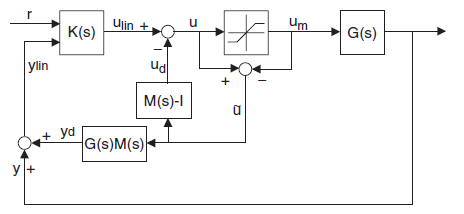
\includegraphics[width=14cm]{figure/chap6/condition_AW.png}
 \label{fig:chap6:F4}
 \bicaption[fig:chap6:F4]{补偿器的具体化}{补偿器具体化} {Fig.}{Conditioning anti-windup compensator}
\end{figure}

对补偿器的表达进一步具体化,可以将抗饱和补偿器表达成一个传递函数的形式。这样,抗饱和补偿器可以使用传递函数矩阵$M(s)$ 进行参数化,具体可以参考图\ref{fig:chap6:F4}。其中系统是用$G(s)$表示,控制器使用$K(s)$表示,参考命令为$r(t)$, 系统的输入为$u_m(t)$,非受限制控制器的输出为 $u(t)$。通过进行参数化,可以进一步将系统进行解耦,其中包括名义线性闭环、非线性闭环以及干扰过滤器三个部分。这个解耦后的框架非常有用,对于后续的抗饱和控制分析与设计非常有用。
\begin{figure}[!htp]
\centering
 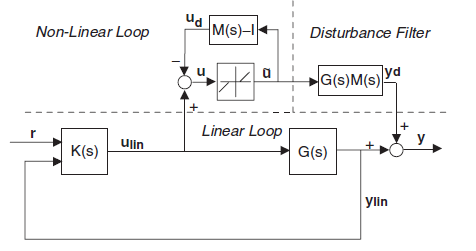
\includegraphics[width=14cm]{figure/chap6/decoupAW.png}
 \label{fig:chap6:F5}
 \bicaption[fig:chap6:F5]{解耦后的补偿控制框架}{解耦后的补偿控制框架} {Fig.}{Decoupled framework of anti-windup compensator}
\end{figure}

从图\ref{fig:chap6:F5}中,可以发现如果从$u_{lin}$ 到$y_d$的映射足够小,那么设计的好的抗饱和补偿器的目标就可以被满足。这个缩小$T_p:u_{lin}\mapsto y_d$的$L_2$增益的问题已经被Turner研究,并且基于LMI优化方法给出了静态、低阶和全阶补偿方法\cite{sofrony2010anti,galeani2009tutorial}。不过这样的方法存在的问题是低阶和静态补偿并不能保证系统的全局稳定性。对于全阶系统,抗饱和补偿器是可以让线性系统镇定,即使是系统处在开环的状态。本章主要研究的也是全阶系统的补偿器。抗饱和补偿器是与鲁棒控制器$K(s)$是独立不相关的,补偿器和系统的关系式如下:
\begin{equation}
\label{eq:chap6:awNs}
G(s) = N(s)M(s)^{-1}
\end{equation}
式中,$N(s)$ 是干扰部分。

基于此可以进一步给出 $M$ 和 $N$ 具体表达式:

\begin{equation}
\label{eq:chap6:awks}
\begin{bmatrix}
\Theta_1  \\
\Theta_2  \\
\end{bmatrix}
=\begin{bmatrix}
M-I	  \\
N     \\
\end{bmatrix}
\sim
\left\{\begin{matrix}
 \dot x &=& (A+BF)x+B \tilde{u }  \\
 u_d &=& F x    \\
 y_d &=& (C+DF)x +D \tilde{u}     \\
\end{matrix}\right.
\end{equation}
式中,$F$ 是自由参数, $A+BF$ 是$Hurwitz$矩阵。这样设计全阶抗饱和补偿器的问题就变成了计算互质分解问题,也就是选择合适的状态反馈增益矩阵 $F$。

标准抗饱和问题的稳定性和性能是通过求解$T_p: u_{lin} \mapsto y_d$ 的增益 $L_2$ 的最小值问题。最小值的代价函数形式如下
\begin{equation}
\label{eq:chap6:costfunction}
L(x,u_{lin},\tilde{u},F,W) = L_a + L_b + L_c
\end{equation}
式中,
\begin{equation}
\begin{aligned}
\label{eq:chap6:La}
L_a =& x^{'} (C^{'}C + A^{'}P + PA + PBZ^{-1} B^{'} P \\
&- PB(WZ^{-1} - I)^{'} W^{-1} Z W^{-1} (W Z^{-1} - I)B^{'}P)x \\
\end{aligned}
\end{equation}

\begin{equation}
\begin{aligned}
\label{eq:chap6:Lb}
L_b &= \left \| Z^{-1/2}WF - Z^{1/2}W^{-1}(WZ^{-1}-I)B^{'}Px \right \| ^{2}
\\
\end{aligned}
\end{equation}

\begin{equation}
\begin{aligned}
\label{eq:chap6:Lc}
L_c =& - \left \|Z^{1/2}\tilde{u} - Z^{-1/2}(B^{'}P-WF)x\right \|^{2}  \\
& - \left \|\gamma u_{lin}-\gamma^{-1} W \tilde{u}\right \|^{2}
\\
\end{aligned}
\end{equation}
代价函数主要由三个部分组成,最后一项 $L_c$ 是负的二次项,关键就是让 $L_a$ 和 $L_b$ 等于零,这样可以让代价函数小于零。 令 $L_b = 0$, 则可以得到增益矩阵 $F$。
\begin{equation}
\label{eq:chap6:F}
\begin{aligned}
(Z^{-1/2}WF - Z^{1/2}W^{-1}(WZ^{-1}-I)B^{'}P)=0 \\
\Leftrightarrow\\
  F = (\gamma ^{-2}I - W^{-1}) B^{'}P\\
\end{aligned}
\end{equation}

为令 $L_a = 0$,如果 $P = P^{'}>0$ 这个条件成立,那么就可以求解 $L_a = 0$ 中的Ricatti方程如下:
\begin{equation}
\label{eq:chap6:ricatti}
\begin{aligned}
C^{'}C &+ A^{'}P + PA + PBZ^{-1} B^{'} P \\
&- PB(WZ^{-1} - I)^{'} W^{-1} Z W^{-1} (W Z^{-1} - I)B^{'}P = 0
\end{aligned}
\end{equation}

经过代数简化,可以获得
\begin{equation}
\label{eq:chap6:ricatti_simple}
C^{'}C + A^{'}P + PA + \gamma ^{-2}PBB^{'}P = 0
\end{equation}

这样就可以获得最优补偿器的解,并确保渐进稳定性并可以保证系统的稳定性,并可以给出补偿器的稳定性与鲁棒性定理如附录定理\ref{app_A:thm:2},全阶补偿器是存在的,并且可以选择合适矩阵增益 $F$ ,其中对称正定矩阵$P$可以通过求解代数Riccati方程获得。

%%%%%%%%%%%%%%%%%%%%%%%%%%%%%%%%%%%%%%%%%%%%%%%%%%%%%%%%%%%%%%%%%%
% \subsection{$w$抗饱和补偿器 }

% 在实际系统中,驱动器阈值是一个非常重要的非平滑非线性,这在工业控制中是比较平常的现象。在控制设计时,如果忽略阈值特性,就会严重的降低控制器的工作性能。基于Riccati方程的驱动补偿器方案中,补偿器的输入是无限制控制输出信号和驱动器阈值输入信号之间的差值,补偿器的输出有两个,一个是状态补偿,一个是控制补偿。但是要解决输入阈值问题,并不是所有的补偿都必须的,借助于状态补偿可以设计辅助设计系统补偿方案如图\ref{fig:chap6:aux}。

% \begin{figure}[!htp]
% \centering
%  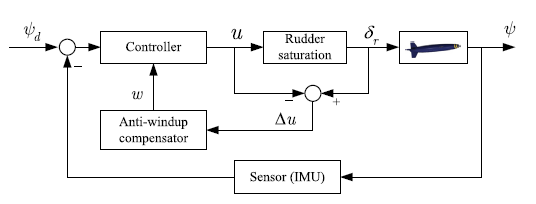
\includegraphics[width=14cm]{figure/chap6/auxilarysystem.png}
%  \label{fig:chap6:aux}
%  \bicaption[fig:chap6:aux]{辅助补偿器}{辅助补偿器.} {Fig}{Auxiliary anti-windup compensator.}
% \end{figure}

% 为了分析输入阈值限制特性的方便,设计辅助补偿器方案如下\cite{Chen2009Neural,galeani2009tutorial}:
% \begin{equation}
% \label{eq:chap6:aux}
% \dot w = \left\{ {\begin{array}{*{20}{c}}
%    { - {k^ * }w - \frac{{\left| {{{\bar c}_3}} \right| + \frac{1}{2}{{\left( {\Delta u} \right)}^2}}}{{{{\left| w \right|}^2}}}w + \Delta u,} & {\left| w \right| \ge l}  \\
%    {0,} & {\left| w \right| < l}  \\
% \end{array}} \right.
% \end{equation}
% 式中,$\Delta u = {\delta _r} - u$ , $w$ 是辅助设计系统的状态, ${k^ * } > 0$ 是设计的参数, $l$ 是正常数, 具体控制方案可以参考图\ref{fig:chap6:aux}。需要指出的是辅助系统补偿方案是符合系统的Lyapunov稳定原理的,补偿器和系统控制器的结合是可以保证整体系统的近似稳定性的。
% \subsection{正 $\mu$ 修改补偿控制方案  }

% \subsection{LMI不等式的补偿控制 }


\section{带有驱动补偿的鲁棒自适应控制  }

\subsection{带有补偿器的模型参考自适应控制  }

在存在有界干扰的情况下,受噪声影响时控制器的参数漂移。然而漂移问题可以使用基于投影算子的自适应算子控制律来解决,可以保证自适应控制律的有界性,进而保证鲁棒自适应控制的稳定性。带有驱动补偿的鲁棒自适应控制,本质上是对原有框架的一种优化,因此其可以保持水下机器人系统以及相应的误差动态的闭环稳定性。由于补偿器会产生状态输出信号,自适应更新律需被重写:

\begin{equation}
\label{eq017}
\begin{array}{l}
{\dot{\hat{\bm K}}_x (t)}=Proj(\hat{\bm K}_x(t),-\bm{\Gamma}_x (\bm{x}(t) + x_{aw}) {\bm e}(t)\bm{PB}sgn(\bm \Lambda)) \\
{\dot{\hat{\bm K}}_r (t)}=Proj(\hat{\bm K}_r(t),-\bm{\Gamma}_r \bm{r}(t) {\bm e}(t)\bm{PB}sgn(\bm \Lambda))
\end{array}
\end{equation}

可以给出鲁棒模型参考自适应的控制律如下:

\begin{equation}
\label{eq014}
u = \hat{\bm{K}}_x ^{T}(t)(\bm{x}(t) + \bm{x}_{aw}) + \hat{\bm{K}}_r ^{T}(t)\bm{r}(t) - u_{aw}
\end{equation}
其中,$\hat{\bm{K}}_x$, $\hat{\bm{K}}_r$分别是与状态与输入有关的更新律通过迭代估计获得的相对应的参数。



% 这一部分给出了所提出控制方法应用于潜水控制系统的不同系统模型的控制仿真结果。



% 所提出的控制器是基于REMUS AUV的6自由度平台,使用matlab/simulink进行测试的。测试主要分为两个模型进行的,一个工厂模型是简化的深度模型,另一个是直接使用6自由度实验模型。鲁棒模型参考自适应控制器相关的参数给出如下:M1系统的相关控制器参数:A= [], B = [], A_ref=[], B_ref = [], Prb_x, Prb_r, Gamma . 补偿器的参数coefficient_rou = 0.01 ; coefficient_W   = 1; coefficient_e   = 0.1,补偿器的区间范围[],其中、delta 为中心值. M2 系统的控制使用的是PD控制,参数如下:.

\subsection{带有补偿器的$L_{1}$自适应控制 }

在这一部分中,现代抗饱和方案扩展到$L_1$自适应控制器。为了加强控制器在实际应用中的可行性,考虑了驱动器饱和问题。 最近,一些现代抗饱和(AW)补偿器已被用于处理输入饱和。然而,线性矩阵不等式(LMI)的大多数解决方案都容易出现数值误差\cite{galeani2009tutorial}。而且,抗饱和补偿器控制器的鲁棒性不太受关注。我们需要的补偿器是可以在发生饱和时优化控制器的性能。基于Riccati的抗饱和补偿器被提出来减少解决LMI问题的计算负担\cite{galeani2009tutorial,folcher2004lmi}。所提出的控制器的框图如图\ref{fig:chap6:F6}所示。

如图\ref{fig:chap6:F6}所示,当驱动器的饱和被激活时,补偿器产生两个不同的输出。一个反馈到控制律,另一个用于修改控制信号。


抗饱和问题被转化为状态反馈的形式,由下式给出:
\begin{equation}
\begin{array}{l}
 {{\dot x}_{aw}} = (A + BF){x_{aw}}(t){\rm{ + }}B\tilde u \\
 {u_{aw}} = F{x_{aw}}(t) \\
 {y_{aw}} = (C + DF){x_{aw}}(t) + D\tilde u \\
\end{array}
\end{equation}
其中, $x_{aw}$ 和 $u_{aw}$ 是抗饱和补偿器的两个输出; $y_{{aw}}$是补偿器测量的输出; $F$是一个自由参数,而 $A+BF$ 必须是 $Hurwitz$ 。 因此,设计一个全阶抗饱和补偿器的问题变成了选择一个适当的状态反馈增益矩阵 $F$ 的问题。

驱动器输入偏差给出如下:
\begin{equation}
\label{eq:8-1}
\tilde u = {u_c}(t) - u(t)
\end{equation}

考虑到驱动器输入饱和,驱动器的非线性函数给出如下:
\begin{equation}
\label{eq:8-2}
u(t) = sat({u_c}(t),{u_{\max }})
\end{equation}

在等式\ref{eq:8-1}和\ref{eq:8-2}中,$u_c(t)$ 是$L_{1}$自适应控制器的控制信号输出,$u(t)$是补偿器的驱动器或推力输出信号,$u_{max}$ 是最大适用控制信号。 抗饱和补偿器输出信号的具体形式表示为

\begin{equation}
u(t) = \left\{ {\begin{array}{*{20}{c}}
   {{u_c}(t),} & {if\left| {{u_c}(t)} \right| \le {u_{\max }}}  \\
   {{u_{\max }}sign({u_c}(t)),} & {if\left| {{u_c}(t)} \right| > {u_{\max }}}  \\
\end{array}} \right.
\end{equation}

通过计算如下Riccati方程获得反馈增益矢量$F$:

\begin{equation}
\begin{array}{l}
 {A^T}{P_{AW}} + {P_{AW}}A - {P_{AW}}BR{B^T}{P_{AW}} + {C^T}C = 0 \\
 F =  - (\rho  + \frac{{{W^{ - 1}}}}{\varepsilon }){B^T}{P_{AW}} \\
\end{array}
\end{equation}
其中, $\rho$,$W$ 和 $\varepsilon$ 是抗饱和补偿器的参数。 前文已经对这些参数的稳健分析进行了研究。本文将基于Riccati的抗饱和补偿器扩展到$L_{1}$自适应控制架构中,以修改控制信号,如下所图\ref{fig:chap6:F6}示。
\begin{figure}[!htp]
 \centering
 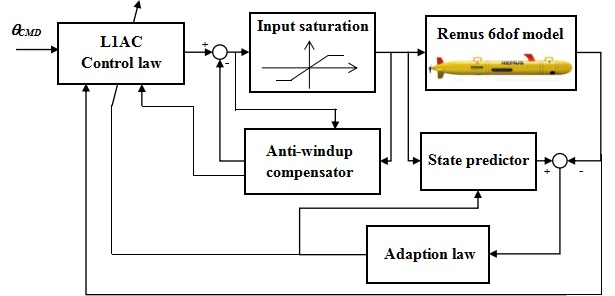
\includegraphics[width=15cm]{figure/chap6/F1.jpg}
 \label{fig:chap6:F6}
 \bicaption[fig:chap6:F6]{带有抗饱和补偿的REMUS AUV 的俯仰自由度的\texorpdfstring {$L_1$}{}自适应控制框图}{带有抗饱和补偿的REMUS AUV 的俯仰自由度的\texorpdfstring {$L_1$}{}自适应控制框图} {Fig.}{Block diagram of L1AC with AW compensator for REMUS AUV in pitch channel}
 \end{figure}

$L_1$自适应控制可以通过计算自适应律来调整参考模型,也采用了射影算子来确保受到干扰和不确定性时的一致有界性。由于驱动器限制的存在,自适应律需要参考前面的补偿器的架构进行修正。控制器的修改通过在自适应律和控制律中用 $x(t)+ x_{aw}(t)$ 代替 $x(t)$来简单地实现。

\begin{equation}
\begin{array}{l}
 \dot {\hat {\theta }}(t) = {{\boldsymbol{\Gamma }}_\theta } {\rm{Proj}}(\hat \theta (t), - {{\tilde x}^T}(t){\left\| ({x(t)+x_{aw})} \right\|_{{\rm{L}}\infty }}PB) \\
 \dot {\hat {\sigma }}(t) = {{\boldsymbol{\Gamma }}_\sigma } {\rm{Proj}}(\hat \sigma (t), - {{\tilde x}^T}(t)PB) \\
 \dot {\hat {\omega }}(t) = {{\boldsymbol{\Gamma }}_\omega } {\rm{Proj}}(\hat \omega (t), - {{\tilde x}^T}(t)u(t)PB) \\
 \hat {\theta } (0)= {{\hat \theta }_0} \\
 \hat {\sigma } (0)= {{\hat \sigma }_0} \\
 \hat {\omega } (0)= {{\hat \omega }_0} \\
 \end{array}
 \end{equation}
其中,$\boldsymbol{\Gamma} \in {\mathbf{R}}^{ + }$ 是自适应增益。当设定任意对称矩阵 $Q=Q^{T}>0$,对称的正定对角矩阵 $P$ 是李雅普诺夫方程的解 $A_m^TP + P{A_m} =  - Q$ 。 需要注意,$u(t)$ 是驱动器接收到的实际控制输入,而非控制器的输出信号。


在本节中,提出的控制方法将在REMUS水下航行器中实施。 如图\ref{fig:chap6:F6}所示,具有抗饱和补偿器方法的$L_{1}$自适应控制用于利用期望的设定点$\theta{CMD}$来控制REMUS航行器的俯仰自由度。

\begin{equation}
\begin{array}{l}
 {u_a}(s) =  - kD(s)(\hat \mu (s) - {k_g}r(s) - {u_{aw}}(t)) \\
 \hat \mu (s) = \ell \left\{ {\hat \mu } \right\}\mathop  = \limits^{} \ell \left\{ {\hat \omega (t)u(t) + \hat \theta (t){{\left\| {x(t) + {x_{aw}}(t)} \right\|}_{{\rm{L}}\infty }} + \hat \sigma (t)} \right\} \\
 \end{array}
 \label{eq:chap6:24}
\end{equation}
其中, $u(t)$ 是驱动器的输入, 滤波器是通过使用$D(s)= 1/s$来确定,具体由来下文给出。

$L_{1}$自适应控制器需要满足$ L_1 $标准条件以确保系统的稳定性,并且当适当的反馈增益 $k$和滤波器 $D(s)$ 可以被确定时,以下不等式成立。

\begin{equation}
\label{eq:22}
\left \| G(s)_{L_{1}} \right \| L<1
\end{equation}
其中,
\begin{equation}
\label{eq:23}
\begin{aligned}
G(s) &\triangleq H(s)(1-C(s)) \\
H(s) &\triangleq (sI-A_{m})^{-1}b\\
L &\triangleq max{\left \| \theta \right \| _{1} }, {\theta \in \Theta} \\
C(s) &\triangleq \omega \kappa D(s) /(1+\omega \kappa D(s))\\
\end{aligned}
\end{equation}

在公式\ref{eq:23}中, $C(s)$ 是严格定义的闭环动态系统的稳定滤波器,可以用来减弱高频信号的影响。稳定状态的增益常被定义如下$C(0) = 1$。一种直接而有效的选择是$D(s) =  1/s$, 这样可以保证 $C(s)$ 是一个一阶低通滤波器, 具体如下
\begin{equation}
\label{eq:24}
C(s) = {}\frac{\omega k}{s + \omega k}
\end{equation}

由于在抗饱和补偿器融合到$L_{1}$自适应控制框架之后,$A_m$ 和 $D(s)$是恒定的,因此可以看出等式\ref {eq:23}不会改变。因此,带有驱动补偿的控制器可以满足 $L_1$ 标准条件。补偿器只有在 $\tilde u$ 不为零时才会输出信号,这两个信号可用于修正控制器的输出 $u_c$或补偿速度 $q$ 以及俯仰角 $\theta $。在等式\ref {eq:chap5:59}中,通过分析自适应定律和控制定律,用 $x(t)+ x_{aw}(t)$ 替换 $ x(t)$ 可以简单地实现对控制器的修改。由于方程\ref {eq:chap6:24}给出的控制律的值总是小于 $u_c$,这意味着 $u$ 的集合是$u_c$所构成的 集合的一个子集, 所以可以保证$L_{1}$自适应控制器的稳定性。REMUS和线性系统模型已在第四章中给出。在本节中,带有补偿的自适应控制器被应用在REMUS水下航行器上。如图\ref{fig:chap6:F6}所示, 利用带有抗饱和补偿器方法的$L_{1}$自适应控制跟踪期望的设定点 $\theta_{CMD}$ 以达到控制REMUS航行器的俯仰自由度的目的。

\subsection{姿态控制实验 }

%---------------------------------------------------------------------
\begin{figure}[!htp]% 0 0 798 187
\centering
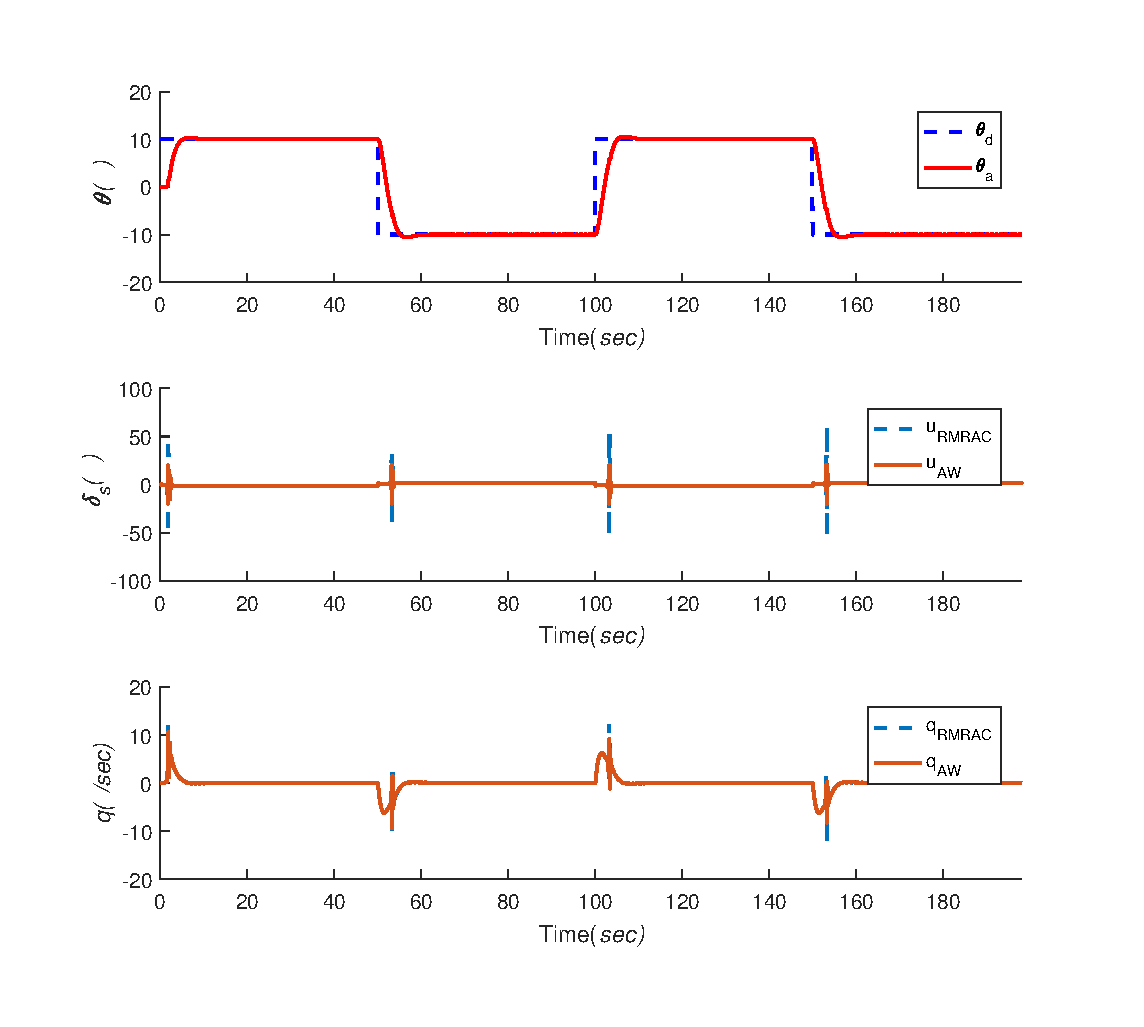
\includegraphics[width=0.85\linewidth]{figure/chap6/Fig1_pulse_theta1.eps}
\label{fig:chap6:F7}
\bicaption[fig:chap6:F7]{存在驱动器阈值补偿的简化潜水系统的鲁棒模型参考自适应的俯仰角跟踪指令$\theta_{d}$}{存在驱动器阈值补偿的简化潜水系统的鲁棒模型参考自适应的俯仰角跟踪指令$\theta_{d}$} {Fig.}{RMRAC control for simplied diving system model in the presence of the actuator saturation when tracking $\theta_{d}$}
\end{figure}

\begin{figure}[h]% 0 0 798 187
\centering
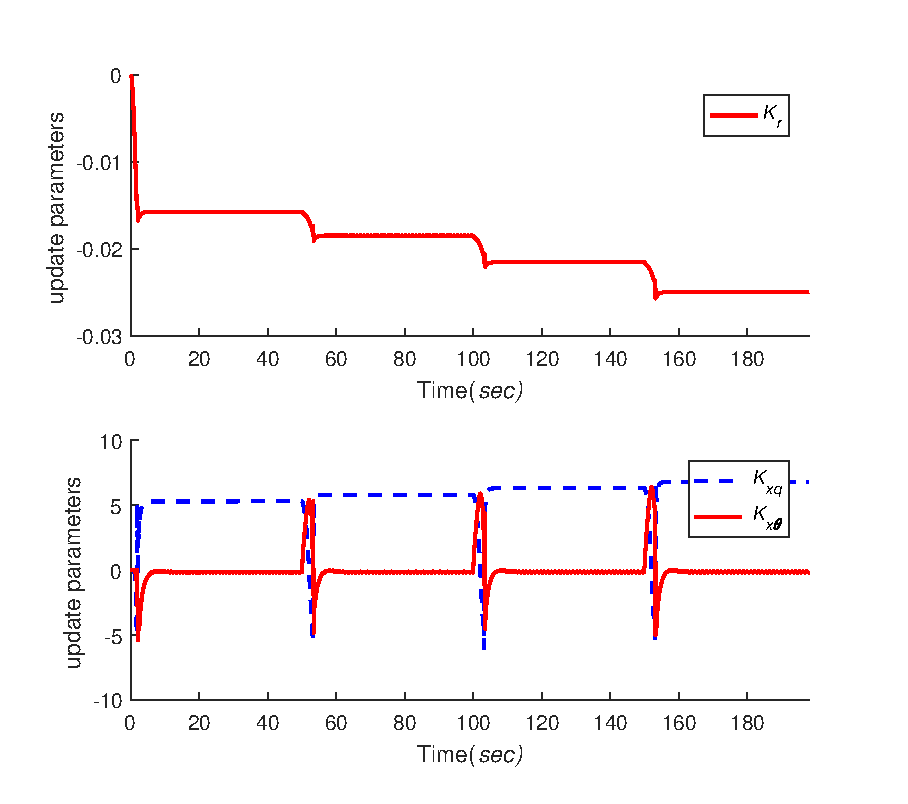
\includegraphics[width=0.85\linewidth]{figure/chap6/Fig1_pulse_theta2.eps}
\label{fig:chap6:F8}
\bicaption[fig:chap6:F8]{带有驱动器补偿的鲁棒自适应控制跟踪$\theta_{d}$时的自适应参数更新}{带有驱动器补偿的鲁棒自适应控制跟踪$\theta_{d}$时的自适应参数更新} {Fig.}{Adaptvie parameters update in RMRAC with an anti-windup compensator when tracking $\theta_{d}$}
\end{figure}
%----------------------------------------------------------------

\subsubsection{带有抗饱和补偿的鲁棒模型参考自适应控制 }
本节给出了不同深潜控制系统模型的控制仿真结果,并将该方法与不同情况下的鲁棒模型参考自适应控制进行了比较。

所设计的控制器是基于REMUS AUV 的6自由度非线性水动力学模型设计的, 并通过使用MATLAB/Simulink实现。在仿真中已经使用了两种用于运载器深度模式的动态系统。 一个是简化的基于线性的深潜模型动态系统,另一个是从实验中提取的6自由度非线性动力学模型\cite{prestero2001verification}。

与鲁棒模型参考自适应控制器相关的参数
给出如下:$ A= [-0.8200,-0.6900; 1.0000,0]$,$B = [ - 4.1600; 0]$,$ A_ {ref} = [ - 1.0900,-0.5200; 1.0000,0]$,$B_ {ref} = [0.5200;0]$。 $K_x$ 和 $K_r$ 的 $\theta_ {max}$ 分别为 $300$ 和 $100$。 对于每个自适应更新规则,投影公差 $\epsilon$ 为 $0.3$,对于每个自适应更新律 $\bm{\Gamma}$ 为 $10$。 在Lyapunov方程中 $\bm {Q} $ 是 $[20,0; 0,200]$。$L_1$控制器的参数可参考第五章。补偿器的参数被定义为:$\rho = 0.01$, $\zeta = 1$ 和 $\varepsilon = 0.1$。 驱动器的数字区间限制在 $-20 + \delta_{s0}$ 到 $20 + \delta_{s0}$度,其中 $\delta_{s0}$ 与水环境有关,并且是 当期望俯仰角为零时的水平方向舵。 PD控制器被用来控制航行器的水下深度,其中 $P$是 $-0.13$,$D$ 是 $-0.001$。

% 图首先给出了简化形式的深度系统的鲁棒模型参考自适应控制在有无补偿器时的控制器效果。两种控制器都能够跟踪期望的姿态控制指令,跟踪所期望的深度指令。此外,RMRAC和带有补偿的RMRAC控制器水平舵片的输入值结果也被进行了对比。可以看出带有补偿器的控制器可以有效降低输入值,并可以减缓状态响应的超调波动。图给出控制器的自适应参数对比,可以看出当存在干扰时,控制器可以通过自动地调节参数来应对不确定性。

两个控制器都可以遵循所需的命令指令,包括俯仰角和深度。 图\ref {fig:chap6:F7}显示了当跟踪脉冲信号 $\theta_d$时,有和没有两个补偿器的简化深潜模式控制系统的鲁棒模型参考自适应控制的比较结果。 在跟踪 $\theta_{d}$时,图\ref {fig:chap6:F8}的上图、下图依次给出了带有抗饱和补偿器的鲁棒模型参考自适应控制中的自适应参数更新,这表明自适应控制器工作正常。

此外,使用鲁棒模型参考自适应控制和带有抗饱和补偿器的模型参考自适应控制进一步比较,可以发现控制水平方向舵输入(图\ref {fig:chap6:F7})、俯仰角速率以及舵的输入值会适当降低,这将说明了驱动器的阈值非线性在水下机器人控制时出现,并由抗饱和补偿器进行校正。


图\ref {fig:chap6:F9}显示了简化的深潜模式的动态系统模型跟踪期望脉冲深度指令 $Z_d$的控制效果。 图\ref {fig:chap6:F10}提供了当潜水控制系统追踪 $Z_d$时控制器的自适应参数的比较。从上述两图中可以看出,自适应控制器可以通过调整参数自动应对模型的不确定性。

%---------------------------------------------------------------------
\begin{figure}[!htp]% 0 0 798 187
\centering
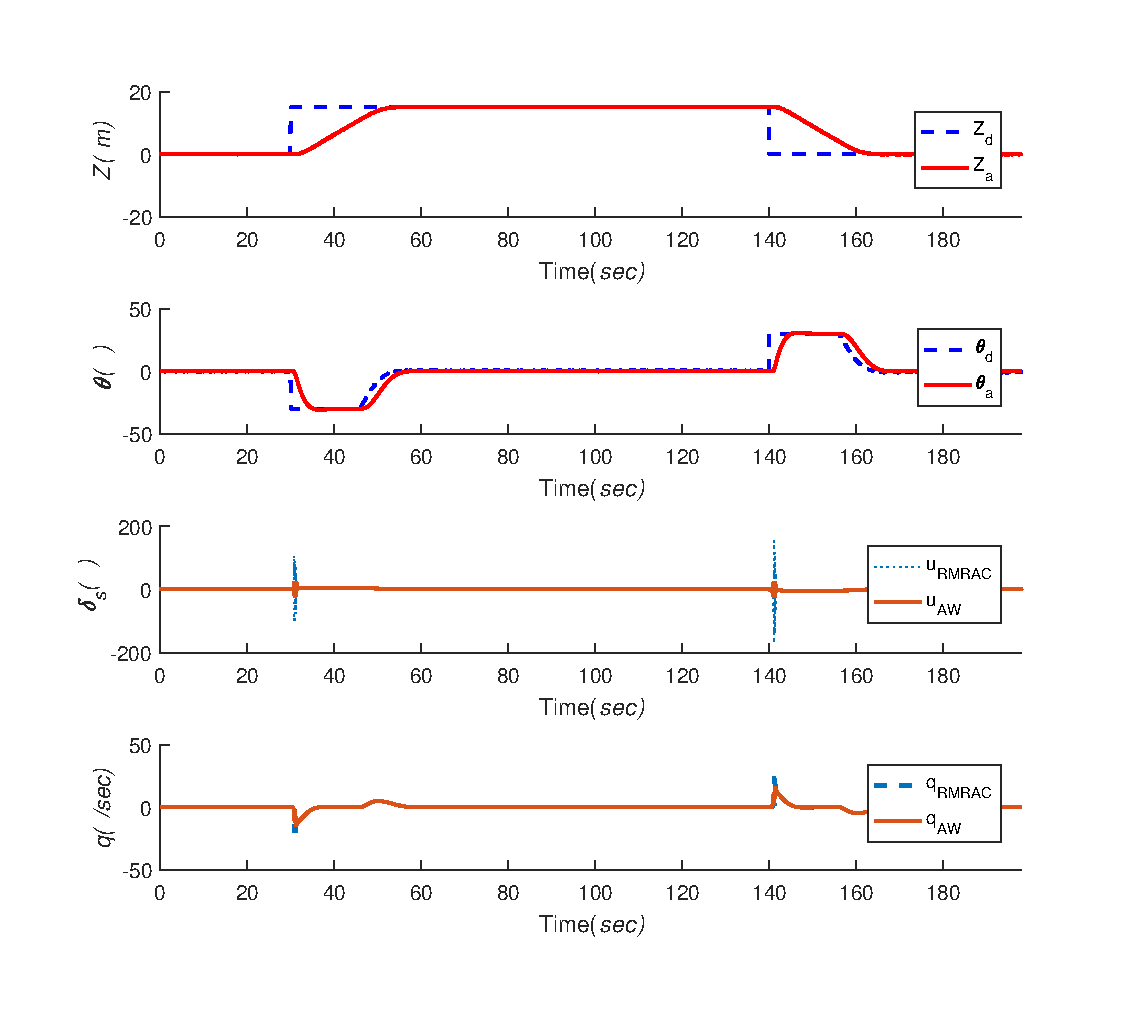
\includegraphics[width=0.85\linewidth]{figure/chap6/Fig_pulsedepth_1.eps}
\label{fig:chap6:F9}
\bicaption[fig:chap6:F9]{存在驱动器饱和的简化潜水系统模型深度$Z_{d}$跟踪控制有无补偿结果对比}{存在驱动器饱和的简化潜水系统模型深度$Z_{d}$跟踪控制有无补偿结果对比} {Fig.}{Comparison of RMRAC control for diving system model tracking $Z_{d}$ with or without anti-windup compensator}
\end{figure}
%----------------------------------------------------------------

\begin{figure}[!htp]% 0 0 798 187
\centering
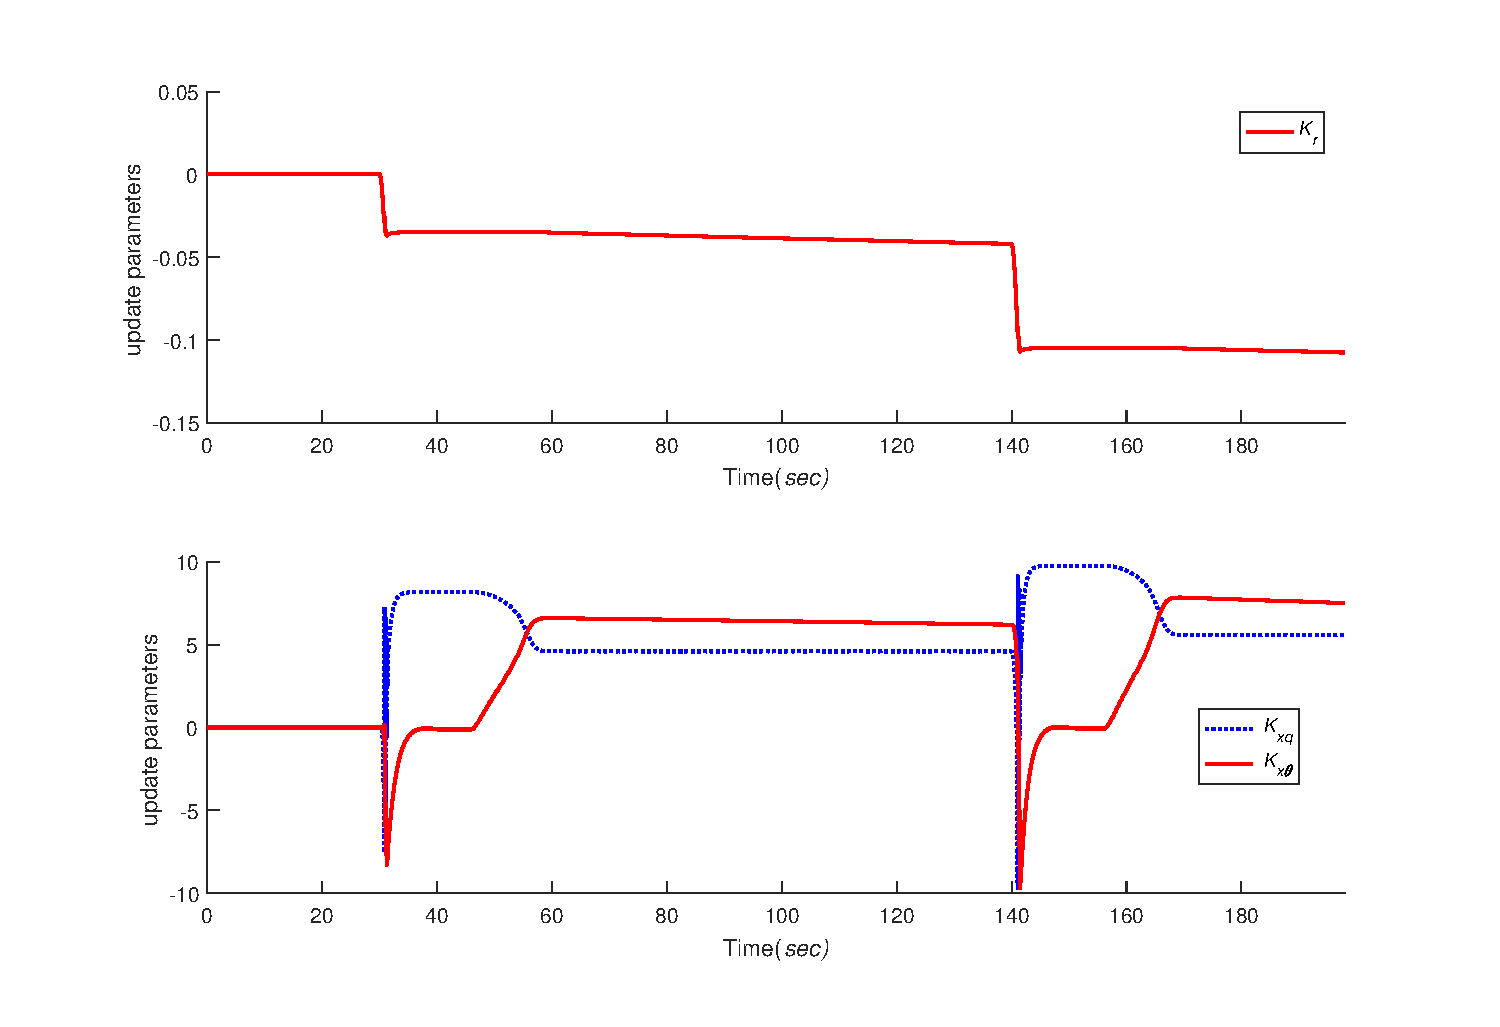
\includegraphics[width=0.85\linewidth]{figure/chap6/Fig_pulsedepth_2.eps}
\label{fig:chap6:F10}
\bicaption[fig:chap6:F10]{带有抗饱和补偿器的鲁棒模型参考自适应控制跟踪$Z_{d}$时的自适应参数更新}{带有抗饱和补偿器的鲁棒模型参考自适应控制跟踪$Z_{d}$时的自适应参数更新} {Fig.}{Parameters updating of the robust model reference adaptive control with anti-windup compensator when the diving system is tracking $Z_{d}$
}
\end{figure}


为了进一步验证所提出的控制器对6自由度模型的控制效果,水下机器人的俯仰角命令被配置在零度上。 因此,可以确定驱动器输入数值区间的中心值。 图\ref {fig:chap6:F11}显示了在不同的水下环境中跟踪所需俯仰角( $\theta_d = 0$)时水下航行器正浮力与稳态误差之间的关系。 通过水下机器人的控制仿真,$\delta_{s0}$ 为 $-0.2$rad 所对应的角度值。

为了进一步研究所提出的控制器应对噪声和干扰的性能,深度模式的干扰在图\ref{fig:chap6:F12}中给出。深度噪声使用噪声功率为8e-5的有界白噪声来定义。

%---------------------------------------------------------------------
\begin{figure}[!htp]% 0 0 798 187
\centering
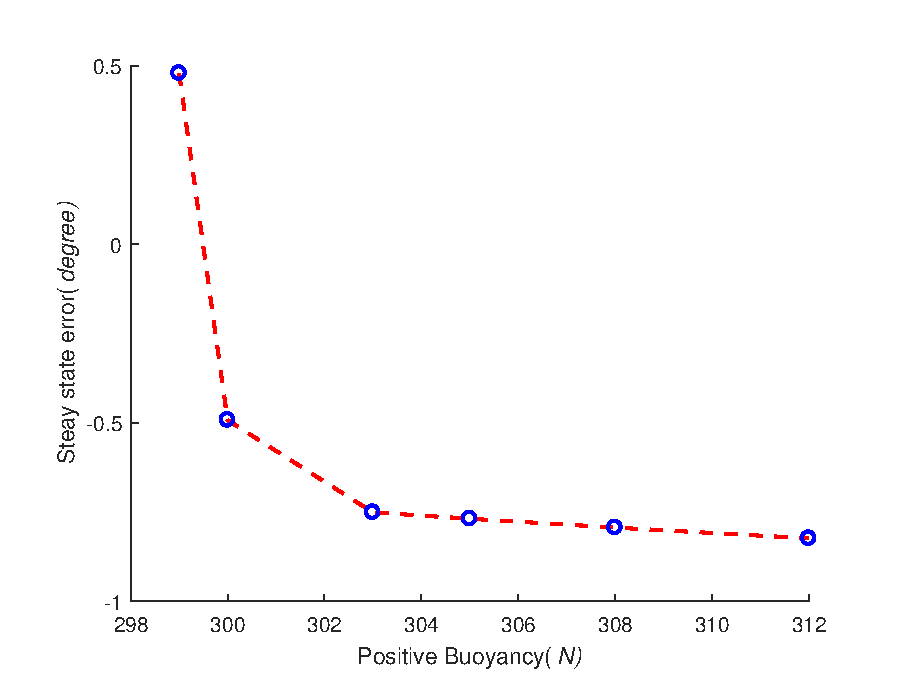
\includegraphics[width=10cm]{figure/chap6/Fig_4.eps}
\label{fig:chap6:F11}
\bicaption[fig:chap6:F11]{正浮力与稳态误差之间的关系}{正浮力与稳态误差之间的关系} {Fig.}{Relationship between the positive buoyancy and the steady-state error}
\end{figure}
%----------------------------------------------------------------

%---------------------------------------------------------------------
\begin{figure}[!htp]% 0 0 798 187
\centering
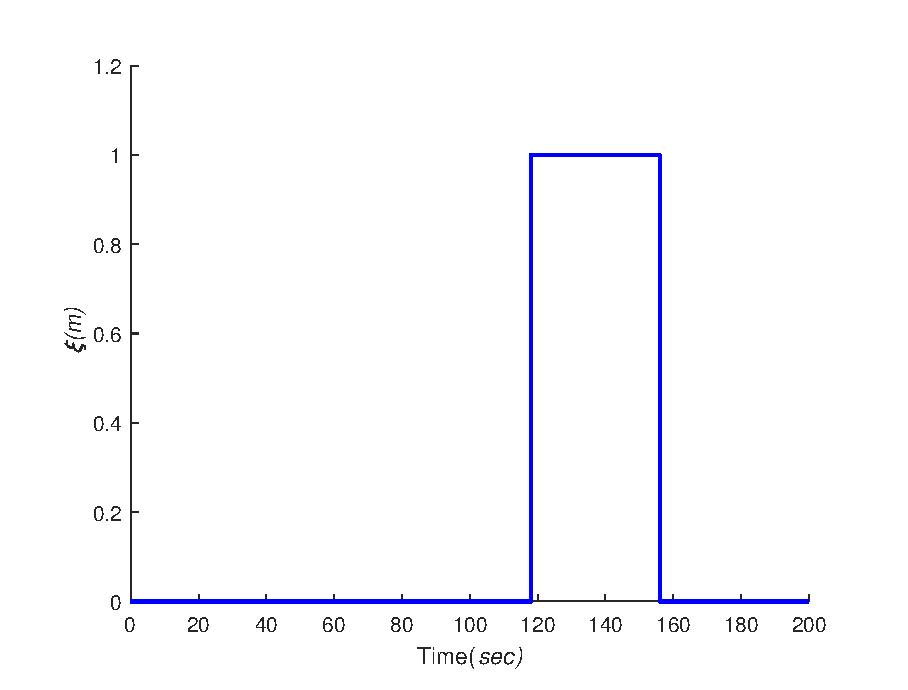
\includegraphics[width=9cm]{figure/chap6/Fig_6_disturbance.eps}
\label{fig:chap6:F12}
\bicaption[fig:chap6:F12]{深度跟踪时的干扰}{深度跟踪时的干扰} {Fig.}{Disturbance $\xi$ in the actual depth $Z_a$}
\end{figure}
%----------------------------------------------------------------


图\ref {fig:chap6:F13}显示了在存在测量噪声和干扰的情况下,6自由度水下自航器跟踪不同深度设置点的追踪效果。 其中带有补偿器的鲁棒自适应控制会因为控制输入的波动小,而对其他自由度(如横滚)的干扰也小(图\ref {fig:chap6:F14})。 然而,由于REMUS AUV的系统是静不平衡的,使用单一舵片来调节具有正浮力的水下机器人模型进行深度追踪时,会出现一定的俯仰角追踪稳态误差。参考方程\ref{depth_equ},可以发现,由于水下机器人要在水下保持稳定,舵片作用力的一个小部分是用来维持水下机器人的垂荡自由度的力平衡。这可以帮助解释为什么姿态角存在稳态误差。

当考虑到噪声和干扰时,在跟踪REMUS航行器的 $Z_{d}$时,图\ref {fig:chap6:F15}给出了在RMRAC中使用抗饱和补偿器的自适应参数更新。它可以揭示出所提出的控制器具有较好的航行器控制能力。然而,带有饱和补偿的鲁棒模型参考自适应控制由于继承了模型参考自适应的控制框架,因此自适应更新慢,稳态误差大这些问题需要深入研究。


%---------------------------------------------------------------------
\begin{figure}[!htp]% 0 0 798 187
\centering
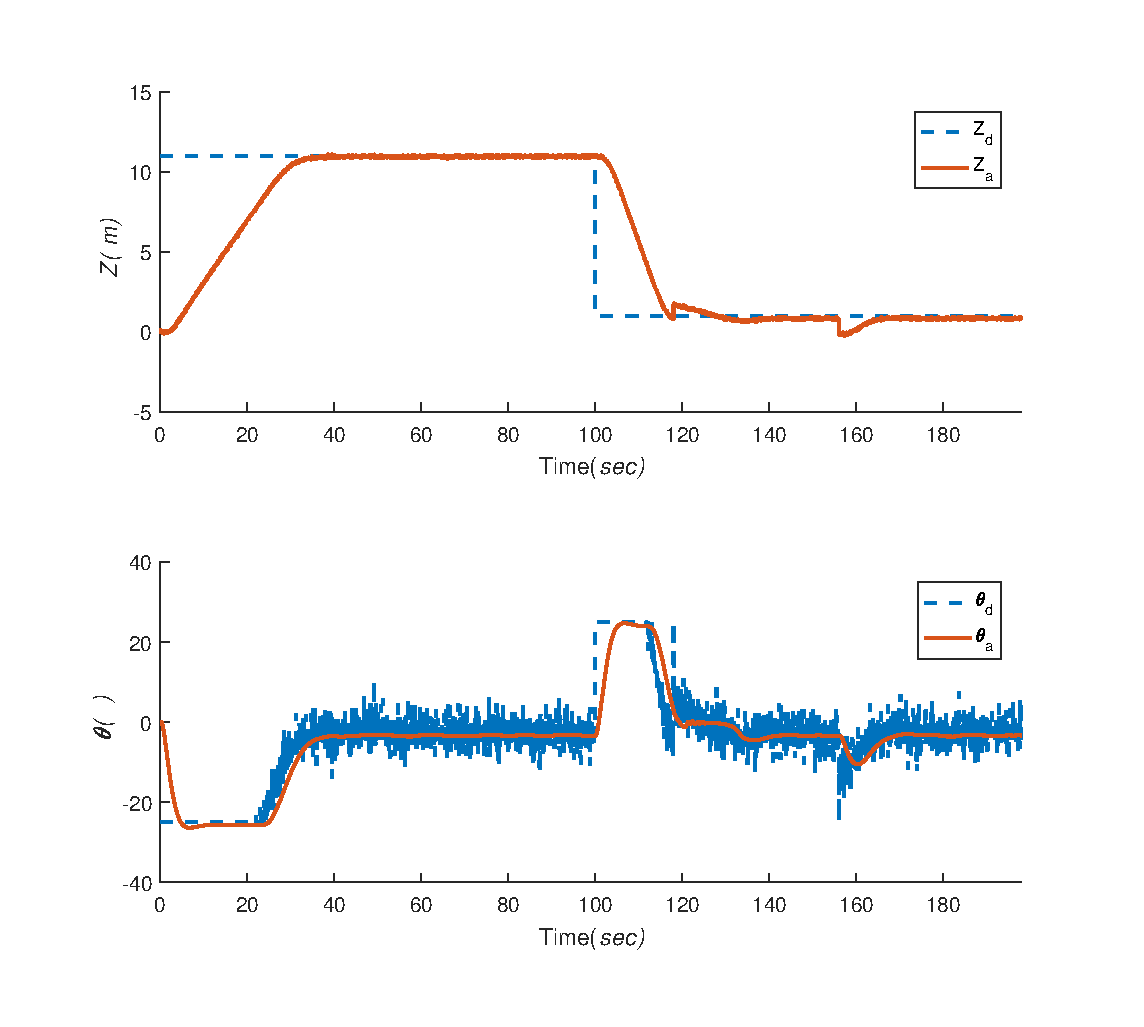
\includegraphics[width=0.85\linewidth]{figure/chap6/Fig6_cmdpulse_1.eps}
\label{fig:chap6:F13}
\bicaption[fig:chap6:F13]{考虑驱动器饱和、测量噪音、干扰 $\xi$ 的REMUS 6DOF模型跟踪的潜水系统深度$Z_{d}$跟踪控制}{考虑驱动器饱和、测量噪音、干扰 $\xi$ 的REMUS 6DOF模型跟踪的潜水系统深度$Z_{d}$跟踪控制} {Fig.}{Diving system control in the presence of the actuator saturation for REMUS 6DOF model tracking $Z_{d}$ with measurement noise disturbance $\xi$}
\end{figure}
%----------------------------------------------------------------

%---------------------------------------------------------------------
\begin{figure}[!htp]% 0 0 798 187
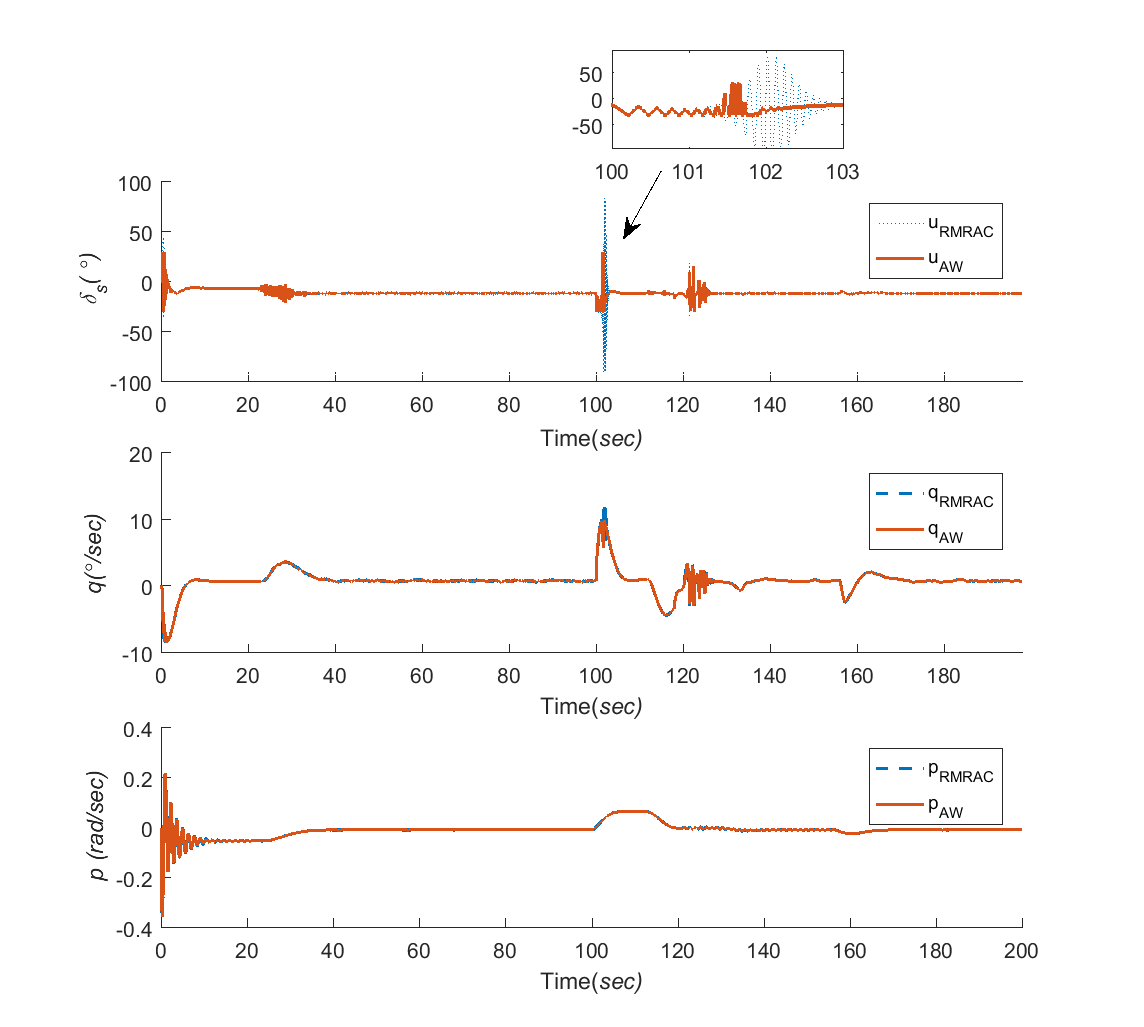
\includegraphics[width=1\linewidth]{figure/chap6/Fig6_cmdpulse_2_mag.eps}
\label{fig:chap6:F14}
\bicaption[fig:chap6:F14]{有抗饱和补偿的RMRAC和无饱和补偿RMARC的驱动器输入、俯仰角和俯仰速率对比} {有抗饱和补偿的RMRAC和无饱和补偿RMARC的驱动器输入、俯仰角和俯仰速率对比} {Fig.}{Actuator input, pitch angle and pitch rate comparisons between RMRAC and RMARC with an anti-windup compensator}
\end{figure}
%----------------------------------------------------------------

%---------------------------------------------------------------------
\begin{figure}[!htp]% 0 0 798 187
\centering
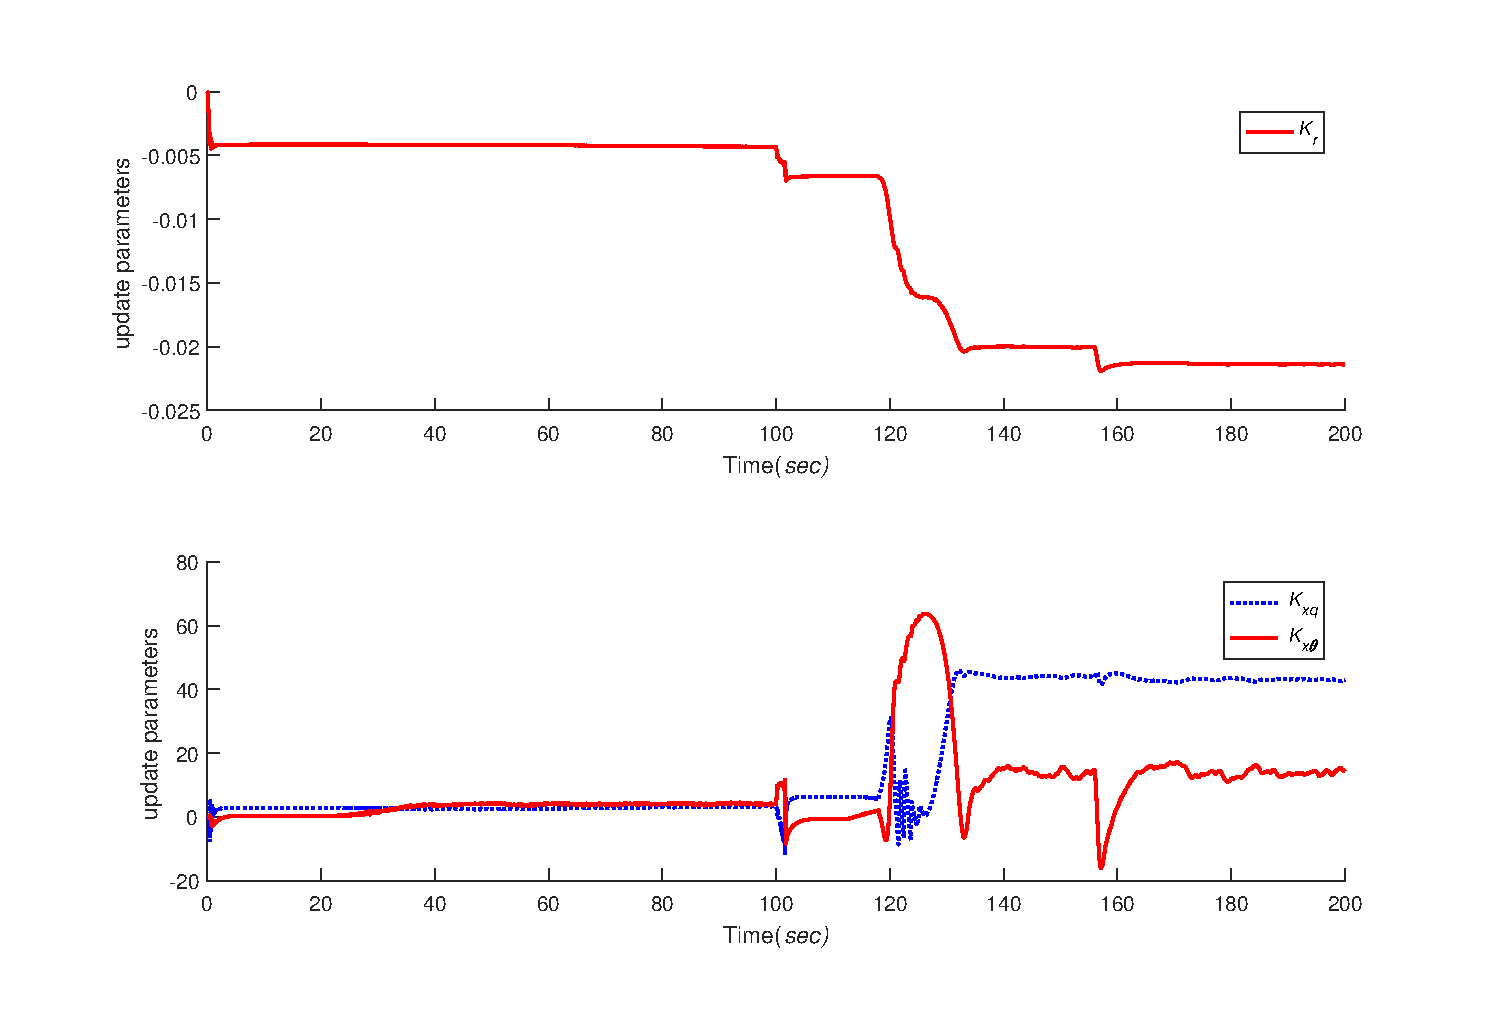
\includegraphics[width=15cm]{figure/chap6/Fig6_cmdpulse_3.eps}
\label{fig:chap6:F15}
\bicaption[fig:chap6:F15]{REMUS 航行器跟踪 $Z_{d}$时带有抗饱和补偿器的鲁棒模型参考自适应控制的自适应参数更新} {REMUS 航行器跟踪 $Z_{d}$时带有抗饱和补偿器的鲁棒模型参考自适应控制的自适应参数更新} {Fig.}{Adaptvie parameters update in RMRAC with an anti-windup compensator when tracking $Z_{d}$ for REMUS vehicle}
\end{figure}
%----------------------------------------------------------------

%----------------------------------------------------------------
\subsubsection{带有抗饱和补偿的$L_1$自适应控制}

用于自适应控制的模型可以通过简化非线性模型获得。然而,航行器控制器的性能很容易受到驱动器的非线性和模型中的不确定性的影响。使用前面提到的带有补偿器的鲁棒自适应控制方法来获得的水下航行器的动态系统模型,并进行仿真。此外,本章还比较了带有或不带有抗饱和补偿器的$L_1$控制器的跟踪性能。

考虑到驱动器的物理空间给输入带来的限制以及控制输入指令的设定要求,驱动器的输入范围应小于最大工作范围。 由于使用不同类型的动态系统模型,用于REMUS俯仰通道的$L_{1}$自适应控制器和抗饱和补偿器的参数不同。REMUS AUV的所有系数都来自Prestero的论文\cite{prestero2001verification}。

在实际实验中,由于螺旋桨的力矩,航行器横滚角并不为零。因此,用水平方向舵控制的俯仰运动与横滚角以及横滚速率是相关的。 在假设REMUS俯仰运动独立的条件下推导出线性动力学模型,这将为航行器控制带来更多的不确定性。 在俯仰角为零时,观察到REMUS航行器在稳定状态下航行时的侧倾角度,$\varphi$,具有平均横滚角偏移约为-5.3度。

\begin{figure}[!htp]
 \centering
 \includegraphics[width=12cm]{figure/chap6/F3_p_roll.eps}
 \label{fig:chap6:F16}
 \bicaption[fig:chap6:F16]{REMUS的6自由度仿真中的横滚角 $\varphi$ 和横摇速率 $p$ }{REMUS的6自由度仿真中的横滚角 $\varphi$ 和横摇速率 $p$ } {Fig.}{Roll angle $\varphi$ and rate $p$ of REMUS in 6DOF model simulation}
 \end{figure}

图\ref{fig:chap6:F16}描述了当螺旋桨力为3.86 N,螺旋桨扭矩为-0.534 Nm时,REMUS航行器的横滚角和横滚速度响应。 横滚自由度与REMUS水下机器人的其他自由度是相互耦合的,可以将其视为俯仰自由度运动控制中的干扰。

\begin{figure}[!htp]
 \centering
 \includegraphics[width=16cm]{figure/chap6/F5_linear_data_control_pitch_new.eps}
 \label{fig:chap6:F17}
 \bicaption[fig:chap6:F17]{存在驱动饱和的线性系统追踪脉冲命令$\theta_{cmd}$的俯仰自由度\texorpdfstring {$L_1$}{}自适应控制}{存在驱动饱和的线性系统追踪脉冲命令$\theta_{cmd}$的俯仰自由度\texorpdfstring {$L_1$}{}自适应控制} {Fig.}{Pitch channel control in the presence of the actuator saturation for linear plant tracking $\theta_{cmd}$(pulse signal) using \texorpdfstring {$L_1$}{} adaptive control }
 \end{figure}

线性系统的动态系统具有不确定性和未知参数主要用于自适应控制,因此研究中不考虑横摇角偏移的影响以及浮力大于重量的影响。 假设的俯仰运动线性模型由 $A_p = [0,1; -0.7,-2]$ 和 $B_p = [0; -4]$。 为了表示在存在输入限制的情况下$L_{1}$自适应控制器的缺点,$L_{1}$自适应控制和所提出的控制器的参考模型如下为 $A_m = [0,1; -9.-4.2]$ 和 $b = [0; - 9]$。 补偿器的参数列出如下:$\rho = 0.01$,$W = 1$,$\varepsilon = 0.1$。 在线性系统的情况下,由于物理空间内输入值的有效性,升降舵角度的输入饱和度被限制在 $-20$ 至 $20$度。

在图\ref{fig:chap6:F17}中,$L_{1}$自适应控制和我们提出的控制器的俯仰角,速率和控制信号在存在模型不确定性和有界干扰的情况下进行比较。 $L_{1}$自适应控制和所提出的方法都可以适应航行器时变不准确的模型参数,但是带有AW补偿器的$L_{1}$自适应控制在性能上优于$L_{1}$自适应控制。应该指出的是,所提出的控制器可以更好地开发航行器驱动器的潜力并减少速度 $q$ 和 $p$ 的波动。

REMUS航行器的6自由度模型是一个强非线性系统,当系统关闭时,由于重力和浮力不能保持稳定,给控制带来更多的不确定性。 在REMUS航行器的俯仰控制情况下,升降舵角度的输入饱和度被限制在 $-20 + \delta_ {s0}$ 到 $20 + \delta_{s0}$ 度,其中$s0$是水平方向舵的输入信号。在仿真中,$\delta_{s0}$ 是 $-0.2$rad所对应的角度值。

鉴于航行器系统控制的电池寿命和整体稳定性,应该仔细考虑输入信号。 如图\ref{fig:chap6:F18}和图\ref{fig:chap6:F19}所示,通过在存在输入饱和的情况下使得舵片的位置在允许范围内,与$L_{1}$自适应控制相比,抗饱和补偿器可以提高$L_{1}$自适应控制的整体性能。

\begin{figure}[!htp]
 \centering
 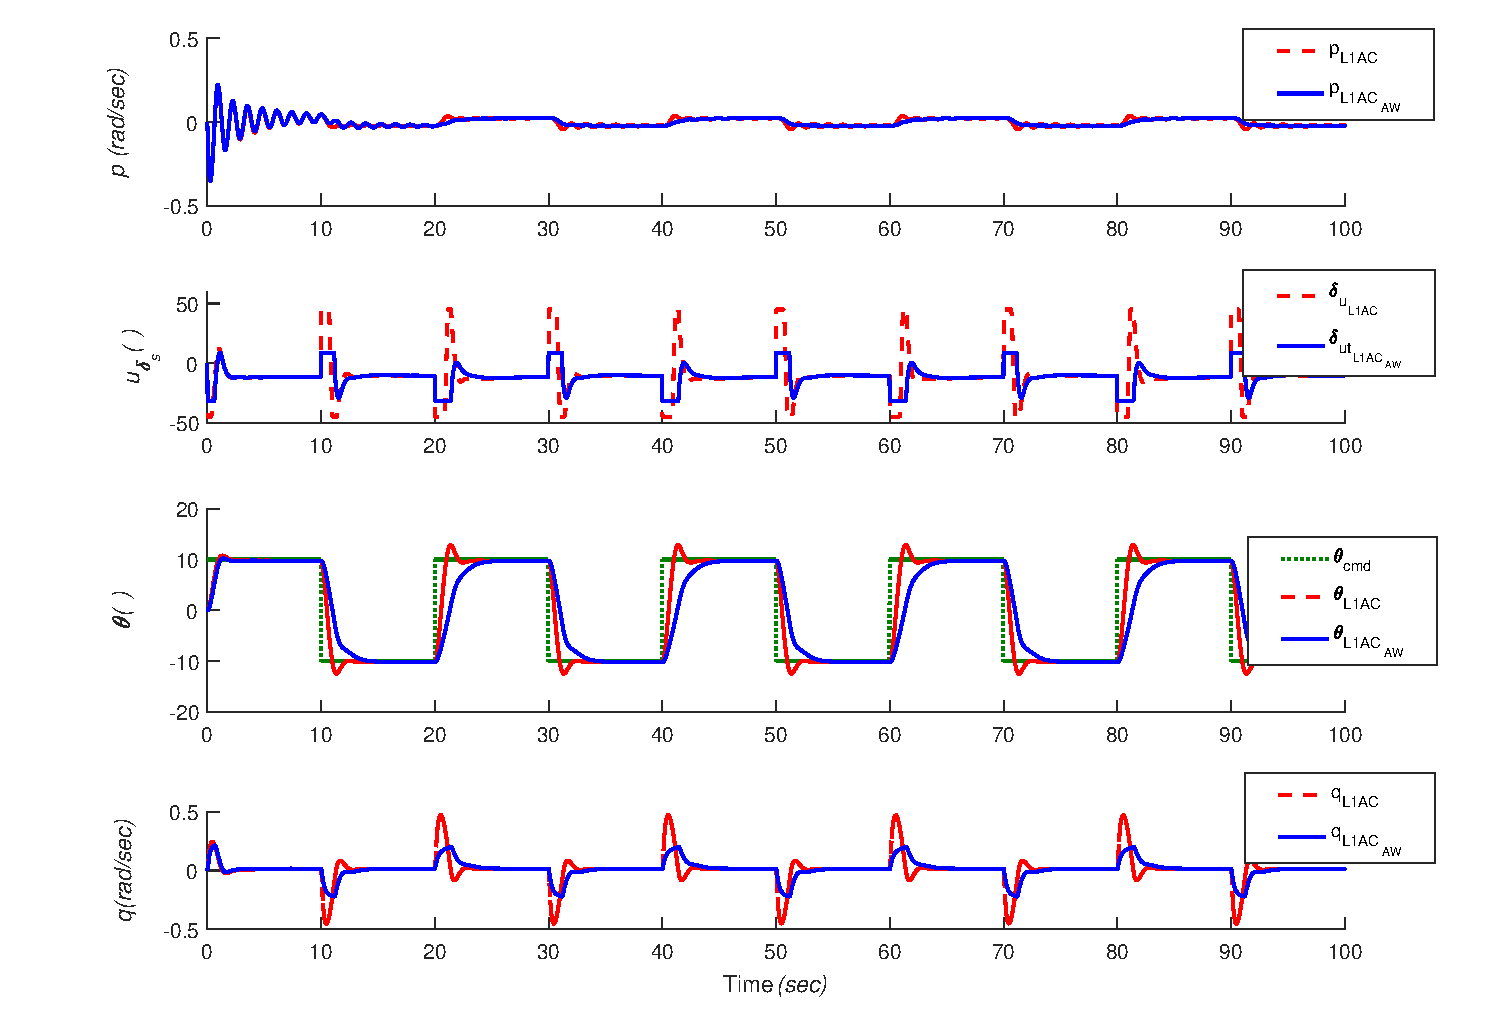
\includegraphics[width=16cm]{figure/chap6/F6_track_10_pluse.eps}
 \label{fig:chap6:F18}
 \bicaption[fig:chap6:F18]{存在驱动饱和的REMUS 6 自由度模型追踪脉冲命令$\theta_{cmd}$的俯仰自由度\texorpdfstring {$L_1$}{} 自适应控制}{存在驱动饱和的REMUS 6 自由度模型追踪脉冲命令$\theta_{cmd}$的俯仰自由度\texorpdfstring {$L_1$} {}自适应控制} {Fig.}{Pitch channel control in the presence of the actuator saturation for REMUS 6DOF model tracking $\theta_{cmd}$(pulse signal) using  \texorpdfstring {$L_1$}{} adaptive control}
 \end{figure}

\begin{figure}[!htp]
 \centering
 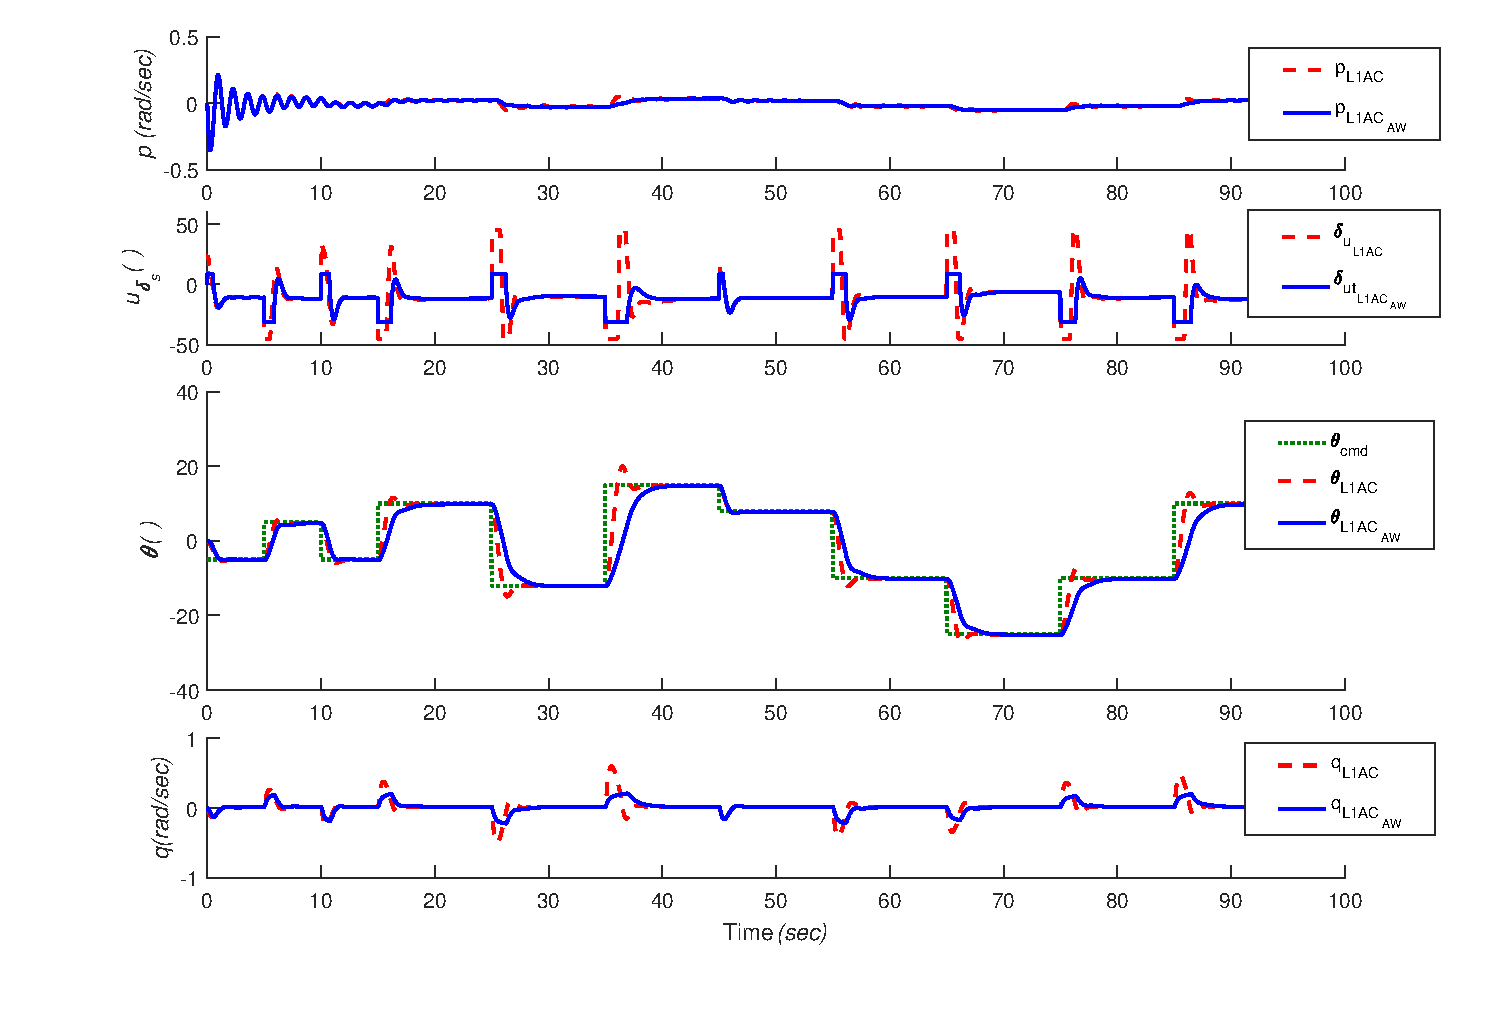
\includegraphics[width=16cm]{figure/chap6/F7_track_signal_builder_nonoise.eps}
 \label{fig:chap6:F19}
 \bicaption[fig:chap6:F19]{存在驱动饱和的REMUS 6 自由度模型追踪不同设定命令$\theta_{cmd}$的俯仰自由度\texorpdfstring {$L_1$}{} 自适应控制}{存在驱动饱和的REMUS 6 自由度模型追踪不同设定命令$\theta_{cmd}$的俯仰自由度\texorpdfstring {$L_1$}{} 自适应控制} {Fig.}{Pitch channel control in the presence of the actuator saturation for REMUS 6DOF model tracking $\theta_{cmd}$ with different set-points using \texorpdfstring {$L_1$}{} adaptive control}
 \end{figure}

 \begin{figure}[!htp]
 \centering
 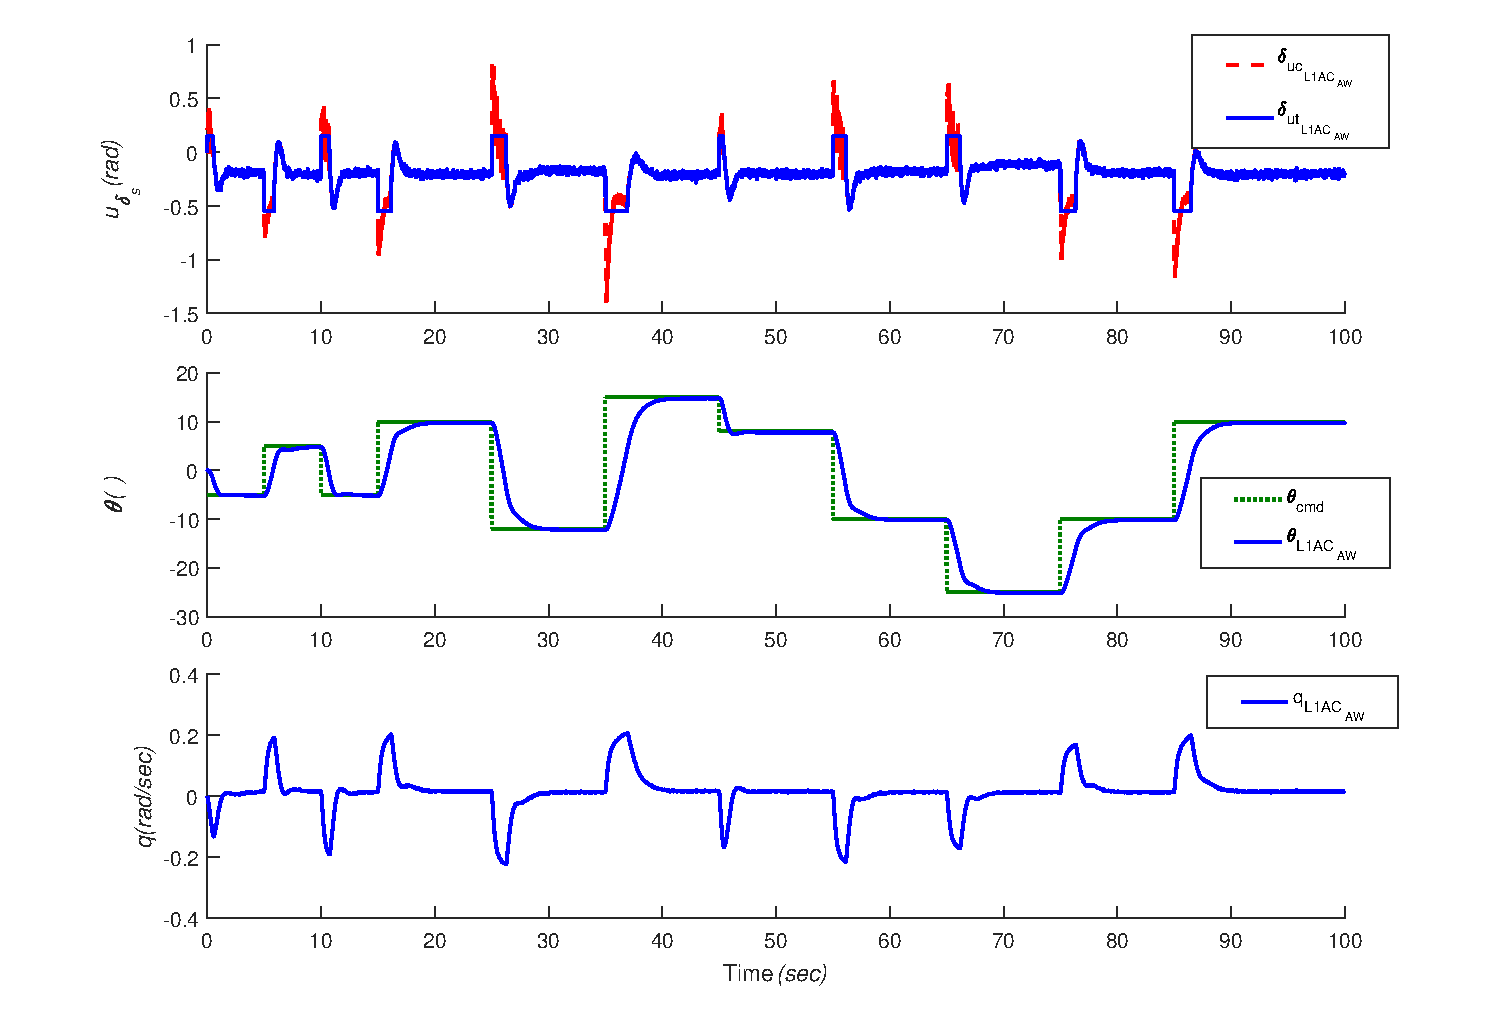
\includegraphics[width=16cm]{figure/chap6/F8_l1aw_withnoise.eps}
 \label{fig:chap6:F20}
 \bicaption[fig:chap6:F20]{存在驱动饱和与噪声的REMUS 6 自由度模型追踪不同设定命令$\theta_{cmd}$的俯仰自由度\texorpdfstring {$L_1$}{} 自适应控制}{存在驱动饱和与噪声的REMUS 6 自由度模型追踪不同设定命令$\theta_{cmd}$的俯仰自由度\texorpdfstring {$L_1$}{} 自适应控制} {Fig.}{Pitch channel control using \texorpdfstring {$L_1$}{} adaptive control in the presence of the actuator saturation for REMUS 6DOF model tracking $\theta_{cmd}$ with different set-points with measurement noise, elevator disturbance as well as input time-delay }
 \end{figure}

由跟踪指令、扰动、未知模型不确定性以及系统耦合效应引起的控制信号,俯仰角和横滚角速率 $p$ 的意外波动可能被削弱。应该注意的是,$L_{1}$自适应控制控制器的整体稳定性不会受到(如图\ref{fig:chap6:F18}、图\ref{fig:chap6:F19}和图\ref{fig:chap6:F20})所扩展的基于Riccati方程的抗饱和补偿器的影响。

此外,REMUS AUV的非线性6自由度模型被设定追踪期望的俯仰角,以进一步研究提出的方法的实际性能。 从图\ref{fig:chap6:F19}可以看出,尽管在6自由度模型仿真中存在横滚角的波动,但带有抗饱和补偿器的$L_{1}$自适应控制可以应对驱动器的非线性,减缓控制信号的波动以及优化在驱动器干扰时的俯仰角跟踪结果 (功率谱密度(PSD)的高度为 $ 2.36e-6$ ),测量噪声(PSD的高度为 $[4.66e-7,8e-6]$)和输入时间延迟(值为 $0.01$ 秒)。 这表明引入的控制策略适用于存在模型不确定性和驱动器阈值式水下航行器的运动控制实践。并且由于$L_{1}$自适应控制方法具有快速自适应的特点,这使得水下机器人可以快速跟踪期望指令而又不会超过最大俯仰角度而造成设备自动关机。

最后,为了进一步说明所提出的控制的可行性,将带有基于Ricctia方程的补偿器的$L_1$自适应控制应用到REMUS AUV的深潜模型控制中,控制效果如图\ref{fig:chap6:F21}所示。可以发现,提出的控制器可以应对来自于噪声(包括驱动器输入噪声、状态测量噪声以及输入指令的噪声)、干扰(包括俯仰角干扰(如图\ref{fig:chap5:F4})、深度干扰(如图\ref{fig:chap6:F12}))以及驱动器的非线性(阈值饱和、时间延迟)。相比于基于模型参考自适应控制的框架,带有补偿器的$L_1$ 自适应控制可以快速的应对不确定性和干扰,并且具有较好的鲁棒性, 稳态误差更小。

 \begin{figure}[htp]
 \centering
 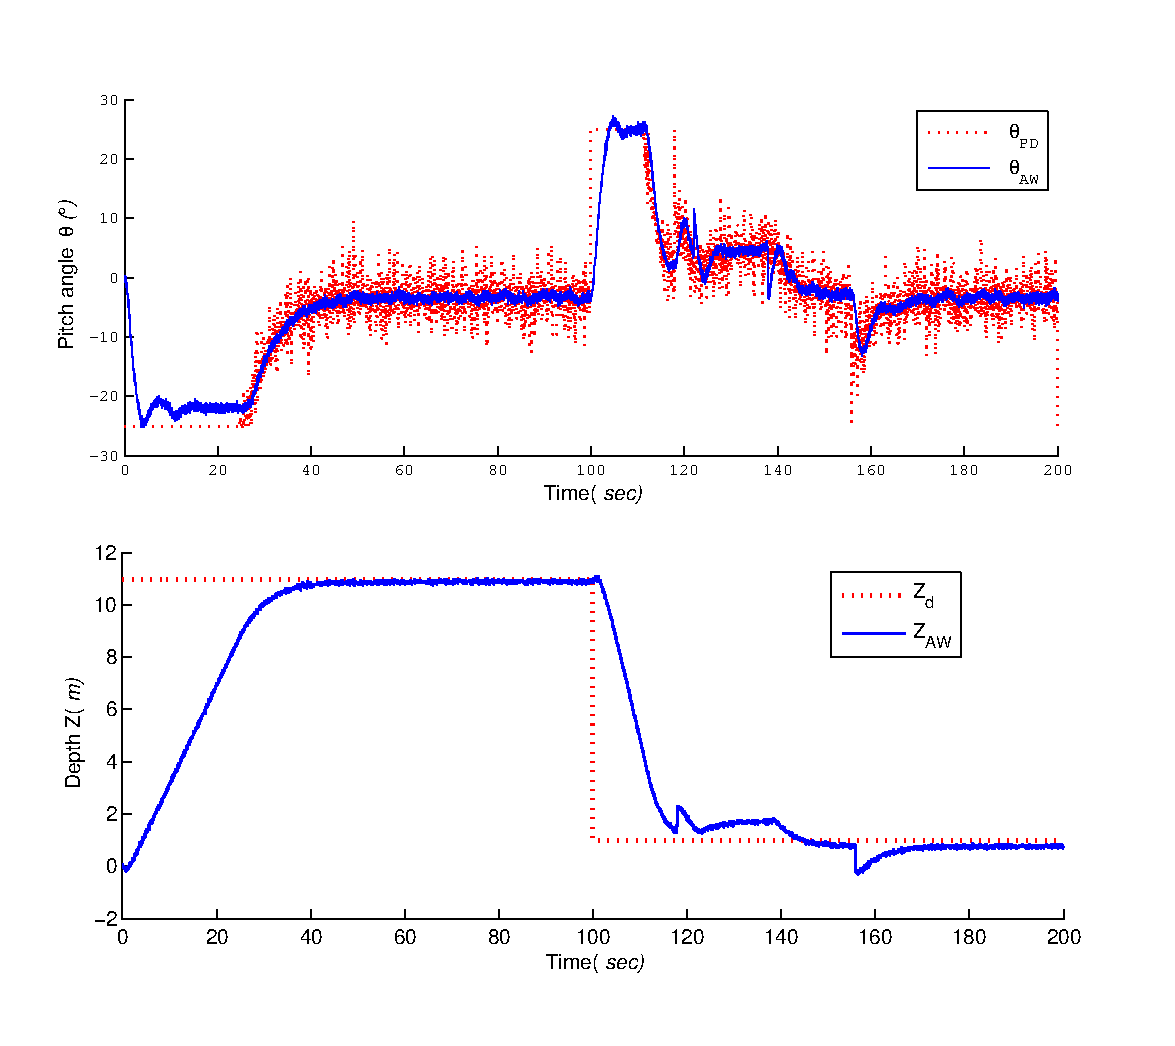
\includegraphics[width=15cm]{figure/chap6/F9_l1aw_withnoise_depth.eps}
 \label{fig:chap6:F21}
 \bicaption[fig:chap6:F21]{存在驱动饱和、噪声与干扰时的REMUS 6 自由度模型追踪期望深度指令\texorpdfstring{$Z_{D}$}的俯仰自由度\texorpdfstring{$L_1$}{} 自适应控制}{存在驱动饱和、噪声与干扰时的REMUS 6 自由度模型追踪期望深度指令\texorpdfstring{$Z_{D}$}的俯仰自由度\texorpdfstring{$L_1$}{} 自适应控制} {Fig.}{Diving mode control using \texorpdfstring{$L_1$}{} adaptive control in the presence of the actuator saturation for REMUS 6DOF model tracking the desired depth $Z_{D}$ with measurement noise, as well as disturbances }
 \end{figure}


% \subsection{3D轨迹追踪实验}



\section{本章小结 }

本章系统地研究了静不平衡水下机器人REMUS AUV的驱动器具有动态特性时的鲁棒自适应控制问题。考虑到水下机器人模型的不确定性和扰动,$L_1$自适应框架被选择为本章主要的研究框架,该方案可以确保系统的鲁棒性和瞬态自适应特性,但是这样的控制方法对于存在于REMUS AUV 中的系统动态并没有加以利用,没有发掘系统动态特性对于系统本身的贡献。针对实际系统中的驱动器非线性的系统特点以及选择的鲁棒自适应控制方案,提出带有驱动补偿的鲁棒自适应控制方法来改善系统的跟踪响应。在本章中,分别介绍了水下机器人实际系统中驱动器的输入阈值、死区、时间延迟的驱动器非线性特点,并分析REMUS AUV驱动器系统中的主要影响因素输入阈值问题。为应对驱动器的输入阈值的挑战,将现代补偿器引入鲁棒自适应框架中,并重点研究了基于Riccati方程的输入补偿器的性能,最终选择将Riccati补偿器融入鲁棒模型参考自适应控制和$L_1$自适应控制方案中。为研究动态补偿的鲁棒控制器在水下机器人中的实际应用效果,提出将带有驱动补偿器的$L_{1}$自适应控制分别用于时变线性系统和具有噪声扰动的REMUS AUV的6自由度耦合模型中。姿态与深度控制实验结果给出了本章提出的带有驱动补偿器的鲁棒自适应控制对于原有控制方案的性能优化的可行性,并从机器人的自身动力学角度进一步利用了驱动器系统动态特性改善$L_1$自适应控制,使得控制研究和动力学研究进行反馈。
